\chapter{Kiến thức nền tảng}
\ifpdf
\graphicspath{{Chapter2/Chapter2Figs/PNG/}{Chapter2/Chapter2Figs/PDF/}{Chapter2/Chapter2Figs/}}
\else
\graphicspath{{Chapter2/Chapter2Figs/EPS/}{Chapter2/Chapter2Figs/}}
\fi
\begin{quote}
	\textit{Chương này trình bày những kiến thức nền tảng của học tăng cường. 
	Trong phần đầu tiên, chúng em trình bày định nghĩa của các thành phần cơ bản trong học tăng cường. 
	Tiếp đó, mô hình ``Markov Decision Processes'' được giới thiệu; mô hình này dùng để mô hình hoá các bài toán học tăng cường khác nhau về chung một ``framework'' cố định.
	Từ đó, ta có thể giải các bài toán học tăng cường bằng cách giải bài toán trên mô hình này.
	Cuối cùng, chúng em trình bày thuật toán ``Q-learning'' - thuật toán học tăng cường được chúng em sử dụng trong bài toán tự động chơi game.}
\end{quote}

\section{Các thành phần cơ bản của học tăng cường}
\subsection{Hệ thống và môi trường}
Trong học tăng cường, thành phần cần ``học'' và đưa ra quyết định được gọi chung là \textit{hệ thống} (agent).
Thành phần này tương tác trực tiếp tới các đối tượng ``bên ngoài'' được gọi là \textit{môi trường} (environment).
Một cách đơn giản, môi trường ở đây chính là những thành phần ``ẩn'' mà hệ thống không kiểm soát trực tiếp được; để thay đổi môi trường, hệ thống phải tương tác với môi trường bằng cách thực hiện hành động.
Sự tương tác này diễn ra tại các mốc thời gian nhất định.
Tại mỗi thời điểm, hệ thống lựa chọn hành động dựa trên những thông tin nhận được từ môi trường.
Những thông tin này bao gồm:
\begin{itemize}
	\item \textbf{Trạng thái} (state): những thông tin về môi trường xung quanh mà hệ thống nhận được. 
	Ví dụ trong đánh cờ, trạng thái có thể là vị trí những quân cờ đang có trên bàn cờ. 
	Môi trường trong bài toán học tăng cường có thể mang yếu tố ngẫu nhiên (stochastic environment): một hành động có thể có dẫn đến những kết quả khác nhau.
	Ví dụ như trong trò chơi đổ xúc xắc, giá trị của xúc xắc là hoàn toàn ngẫu nhiên.
	Vì vậy, nếu môi trường thay đổi dựa vào kết quả của xúc xắc thì trạng thái cũng thay đổi một cách ngẫu nhiên.
	Ký hiệu của trạng thái là $s$.
	\item \textbf{Điểm thưởng} (reward): giá trị số thực mà môi trường trả về cho hệ thống; giá trị điểm thưởng này nói lên độ tốt của một hành động tại một trạng thái nào đó. 
	Với ví dụ đánh cờ, điểm thưởng mà hệ thống có thể nhận được từ môi trường ở cuối ván cờ là +1 nếu hệ thống thắng, -1 nếu hệ thống thua.
	Trong quá trình đánh cờ, điểm thưởng có thể là 0 cho mỗi nước cờ mà hệ thống thực hiện.
	Có thể thấy trong ví dụ này, điểm thưởng không nói rõ nước cờ nào là tốt mà chỉ đánh giá tổng quát cho cả ván đấu.
	Chính vì vậy, điểm thưởng có ý nghĩa khác biệt so với nhãn của phương pháp học có giám sát.
	Tương tự như trạng thái, điểm thưởng cũng có thể ngẫu nhiên.
	Với ví dụ xúc xắc, nếu điểm thưởng là giá trị của xúc xắc thì điểm thưởng là ngẫu nhiên.
	Nếu ta chơi hai lần và thực hiện cùng một hành động tại cùng một trạng thái thì điểm thưởng vẫn có thể khác nhau.
	Điểm thưởng được ký hiệu là $r$. 
\end{itemize}
Từ trạng thái và điểm thưởng nhận được, hệ thống chọn hành động phù hợp để đạt được điểm thưởng cao nhất.

Hệ thống và môi trường tương tác với nhau một cách tuần tự.
Thời điểm tương tác (được ký hiệu là $t$) được đánh số tăng dần: $t = 0, 1, 2,..., T$ (với $T$ là thời điểm kết thúc).
Tại thời điểm $t$, hệ thống nhận được trạng thái hiện tại $\mathit{S_t} \in \mathcal{S}$, với $\mathcal{S}$ là tập các trạng thái có thể có. 
Dựa vào trạng thái nhận được, hệ thống thực hiện một hành động $\mathit{A_t} \in \mathcal{A}$, trong đó $\mathcal{A}$ là tập các hành động có thể thực hiện. 
Hành động này làm cho môi trường thay đổi.
Tại thời điểm $t+1$ sau đó, hệ thống nhận được giá trị điểm thưởng $\mathit{R_{t+1}} \in \mathbb{R}$ cùng với trạng thái tiếp theo $\mathit{S_{t+1}}$.
Giá trị $R_{t+1}$ là điểm thưởng nhận được do hành động $\mathit{A_t}$ vừa làm thay đổi môi trường (chứ không phải tổng điểm thưởng từ lúc bắt đầu).
Quá trình tương tác giữa hệ thống và môi trường cứ tiếp tục lặp lại cho đến khi môi trường trả về trạng thái kết thúc.
Quá trình tương tác này được mô tả trong hình \ref{AgentEnvironment}.

\begin{figure}
	\centering
	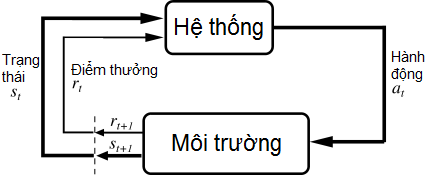
\includegraphics[width=.8\textwidth]{AgentEnvironment}
	\caption{Quá trình tương tác giữa hệ thống và môi trường}
	\label{AgentEnvironment}
\end{figure}

Các thành phần của hệ thống gồm có:
\begin{itemize}
	\item \textbf{Chính sách} $\pi$ là cách hệ thống lựa chọn hành động dựa vào trạng thái hiện tại.
	Tại thời điểm $t$, khả năng một hành động $a$ được chọn ở trạng thái $s$ là $\pi(a \mid s) = \mathbb{P}[\mathit{A_t} = a \mid \mathit{S_t} = s]$. 
	Nếu chính sách luôn chọn một hành động với xác suất là $1$ thì chính sách đó gọi là \textit{đơn định} (deterministic).
	Chính sách đơn định lúc này có thể coi là một ánh xạ từ tập trạng thái sang tập hành động: $a = \pi(s)$.
	Để đạt nhiều điểm thưởng nhất, hệ thống cần có một chính sách chọn lựa hành động phù hợp. 
	Những phương pháp học tăng cường thường tập trung thay đổi dần dần các chính sách của hệ thống để đạt được mục tiêu trên.
	\item \textbf{Hàm giá trị} dùng để đánh giá trạng thái hoặc hành động tại trạng thái là ``tốt'' đến mức nào.
	Để đánh giá một trạng thái, ta có thể thử tương tác với môi trường và tính tổng điểm thưởng nhận được từ khi gặp trạng thái đó cho đến khi kết thúc.
	Tuy nhiên, do môi trường có thể mang tính ngẫu nhiên, tổng điểm thưởng này có thể khác nhau ở những lần tương tác khác nhau.
	Vì vậy, giá trị trạng thái được định nghĩa là \textbf{kỳ vọng} tổng điểm thưởng (lấy trung bình vô số lần tương tác).
	Lúc này, giá trị của một trạng thái $s$ theo chính sách $\pi$ được ký hiệu $v_{\pi}(s)$ là kỳ vọng tổng điểm thưởng mà hệ thống có thể nhận được bắt đầu từ trạng thái $s$ về sau.
	Lý do có chính sách $\pi$ trong định nghĩa này là do điểm thưởng nhận được sẽ phụ thuộc vào cách hệ thống chọn hành động.
	Tương tự, để đánh giá một hành động tại một trạng thái, ta định nghĩa hàm giá trị hành động.
	Giá trị của việc thực hiện hành động $a$ tại trạng thái $s$ rồi tương tác theo chính sách $\pi$ được ký hiệu $q_{\pi}(s,a)$.
	Giá trị này thể hiện là kỳ vọng tổng điểm thưởng mà hệ thống có thể nhận được kể từ sau khi thực hiện hành động $a$ tại trạng thái $s$ và thực hiện các hành động tiếp theo dựa vào chính sách $\pi$. 
	\item \textbf{Mô hình}. Trong một số bài toán học tăng cường, hệ thống có thể xây dựng mô hình cho riêng mình để mô phỏng lại môi trường. 
	Qua đó cho phép hệ thống có thể suy luận hoặc dự đoán những thông tin của môi trường trong tương lai.
\end{itemize}	

\subsection{Tổng điểm thưởng}
Tổng điểm thưởng (return) $\mathit{G_t}$ xác định lượng điểm thưởng mà hệ thống nhận được kể từ thời điểm $t$ trở đi. 
Ta có thể định nghĩa giá trị này bằng:
\begin{equation}
	\mathit{G_t} = \mathit{R_{t+1}} + \mathit{R_{t+2}} + ... + \mathit{R_{T}}
\end{equation}	
ở đây $T$ là thời điểm cuối cuối cùng hệ thống tương tác với môi trường.
Tuy nhiên, tổng này có thể không hữu hạn nếu như độ dài một lần tương tác không được giới hạn.

Từ đây, ta có thể sử dụng một định nghĩa tổng điểm thưởng luôn hữu hạn:
\begin{equation}
\mathit{G_t} = \mathit{R_{t+1}} + \gamma\mathit{R_{t+2}} + \gamma^{2}\mathit{R_{t+3}} + ... + \gamma^{T-t-1}\mathit{R_{T}} = \sum_{k=0}^{\infty}\gamma^{k}\mathit{R_{t+k+1}}
\end{equation}
Trong đó $\gamma$ là hệ số ``giảm điểm thưởng'' (discount factor) với giá trị $0\leqslant \gamma \leqslant 1$.
Đây là định nghĩa tổng điểm thưởng được dùng trong các bài toán học tăng cường.
Lý do chính để các nhà nghiên cứu chọn định nghĩa này là để đơn giản hoá về mặt toán học.
Tuy vậy, định nghĩa này cũng có một số lợi ích khác.
Nếu như cần dự đoán giá trị tổng điểm thưởng tại thời điểm $t$ (một việc mà ta sẽ phải làm thường xuyên), các giá trị điểm thưởng ở càng xa thì khả năng ta dự đoán đúng càng thấp.
Vì vậy, trọng số của các điểm thưởng ở càng xa thời điểm hiện tại cần phải giảm dần.
Với $\gamma = 0$, hệ thống chỉ quan tâm điểm thưởng ngay lập tức mà không quan tâm về lâu dài.
Ngược lại, $\gamma$ càng gần $1$ thì hệ thống càng quan tâm một cách dài hạn hơn về điểm thưởng.

\section{Mô hình Markov Decision Processes}
%	\begin{itemize}
%			\item Các thành phần MDP
%			\item Ví dụ cho mô hình MDP
%			\item Phương trình Bellman
%			\item Qui trình đánh giá chính sách: Kỹ thuật qui hoạch động
%			\item Qui trình cải thiện chính động: Kỹ thuật qui hoạch động
%	\end{itemize}
\subsection{Định nghĩa mô hình Markov Decision Processes}
Mô hình Markov Decision Processes (MDP) được sử dụng để mô hình hóa bài toán học tăng cường một cách hình thức. 
Cụ thể, MDP là một bộ bao gồm 5 thành phần $<\mathcal{S, A, P, R, \gamma}>$:
\begin{itemize}
	\item $\mathcal{S}$: tập trạng thái hữu hạn có thể có của môi trường.
	\item $\mathcal{A}$: tập hữu hạn những hành động mà hệ thống có thể thực hiện để tương tác với môi trường.
	Tổng quát hơn, tại mỗi trạng thái, hệ thống có thể thực hiện những hành động khác nhau.
	Khi đó, tập hành động tại trạng thái $s$ được ký hiệu là $\mathcal{A}(s)$.
	\item $\gamma$: hệ số giảm điểm thưởng có giá trị thỏa $0\leqslant \gamma \leqslant 1$ thể hiện mức độ tin tưởng về giá trị điểm thưởng nhận được ở tương lai.
	\item $\mathcal{P}$: ma trận xác suất chuyển trạng thái. 
	Trong đó $\mathcal{P}_{ss'}^{a}$ là xác suất chuyển đến trạng thái $s'$ khi hệ thống đang ở trạng thái $s$ và thực hiện hành động $a$.
	\begin{equation}
	\mathcal{P}_{ss'}^{a} = \mathbb{P}[\mathit{S_{t+1}} = s' \mid \mathit{S_{t}} = s, \mathit{A_{t}} = a]
	\end{equation}
	\item $\mathcal{R}$: ma trận điểm thưởng của từng \textit{bộ (trạng thái, hành động)}. 
	$\mathcal{R}_{s}^a$ là giá trị kỳ vọng điểm thưởng nhận được \textbf{ngay lập tức} khi hệ thống thực hiện hành động $a$ ở trạng thái $s$.
	\begin{equation}
	\mathcal{R}_{s}^a = \mathbb{E}[\mathit{R_{t+1}} \mid \mathit{S_{t}} = s, \mathit{A_{t}} = a]
	\end{equation}				
\end{itemize}

\textbf{Ví dụ mô hình MDP của bài toán robot thu gom soda (ví dụ chỉnh sửa từ \cite{sutton1998introduction}):} công việc của robot này là thu lượm những lon soda đã được uống hết trong văn phòng. 
Robot có những cảm biến để xác định những lon soda này, bánh xe và cánh tay để di chuyển và gắp nhặt những lon này bỏ vào thùng. 
Robot hoạt động bằng pin sạc. 
Hệ thống điều khiển của robot có chức năng tiếp nhận những thông tin từ cảm biến để điểu khiển bánh xe và cánh tay. 
Trong ví dụ, chúng em chỉ xét dựa trên mức độ pin hiện tại robot nên quyết định tìm kiếm những lon soda như thế nào.
Tại mỗi thời điểm, robot có thể thực hiện một trong ba hành động: (1) thực hiện tìm kiếm một lon soda, (2) đứng yên và đợi người khác mang lon soda đến cho nó, (3) quay trở lại nơi sạc pin. 
Trạng thái của môi trường được xác định là lượng pin hiện tại của robot. 
Cách tốt nhất để tìm kiếm những lon soda là robot thực hiện hành động tìm kiếm, nhưng việc này sẽ làm giảm dung lượng của pin. 
Ngược lại nếu robot đứng yên và đợi thì dung lượng pin không giảm. 
Mỗi khi dung lượng pin ở mức thấp thì robot sẽ quay lại chỗ sạc pin. 
Trường hợp xấu nhất có thể xảy ra là robot không đủ dung lượng pin để quay lại nơi sạc; khi đó robot sẽ đứng yên và đợi ai đó mang nó đến chỗ sạc. 
Do đó robot cần có một chiến lược phù hợp để đạt được hiệu năng cao nhất có thể.
Hệ thống đưa ra những quyết định dựa trên mức năng lượng pin. 
Mức năng lượng này có thể được xác định hai mức \textit{cao} và \textit{thấp}. 
Khi đó tập trạng thái mà hệ thống có thể nhận được là $\mathcal{S} = \left \{\text{cao}, \text{thấp} \right \}$. 
Những hành động của hệ thống trong ví dụ này được xét đơn giản gồm ba hành động \textit{đợi}, \textit{tìm kiếm} và \textit{sạc pin}. Khi dung lượng pin ở trạng thái cao, hệ thống chỉ thực hiện hai hành động: tìm kiếm và đợi. 
Ngược lại khi ở trạng thái thấp, hệ thống có thể thực hiện ba hành động: tìm kiếm, đợi, và sạc pin.
$$\mathcal{A}(\text{cao}) =  \left \{\text{tìm kiếm}, \text{đợi} \right \}$$
$$\mathcal{A}(\text{thấp}) =  \left \{\text{tìm kiếm}, \text{đợi}, \text{sạc pin} \right \}$$

Khi mức năng lượng pin ở mức cao, nếu robot thực hiện tìm kiếm sẽ có xác suất $\alpha$ năng lượng pin vẫn ở mức cao, và $1 - \alpha$ năng lượng của pin sẽ chuyển về mức thấp. 
Mặt khác, khi mức năng lượng ở mức thấp, nếu robot thực hiện tìm kiếm sẽ có xác suất $\beta$ năng lượng pin ở mức thấp, và $1 - \beta$ chuyển đến mức cao (trường hợp này xảy ra khi dung lượng pin cạn kiệt và cần ai đó mang robot đến chỗ sạc). 
Ngoài ra, mỗi lon soda nhặt được tương ứng với $+1$ điểm thưởng và sẽ bị $-3$ điểm thưởng mỗi khi robot phải cần ai đó mang đến chỗ sạc. $r_{\text{đợi}}$, $r_{\text{tìm kiếm}}$ là số lượng lon soda kỳ vọng mà robot có thể thu gom được trong khi đợi và tìm kiếm. Hình \ref{graphRobot} minh họa cho mô hình MDP trong ví dụ robot thu gom lon soda.

%% Hình vẽ
\begin{figure}
	\centering
	\begin{tikzpicture}[node distance=6.5cm,>=stealth',bend angle=45 ,auto]
	
	\tikzstyle{state}=[circle,thick,draw=blue!75,fill=blue!20,minimum size = 15mm]
	\tikzstyle{action}=[circle,draw=black!75,
	fill=black!75,minimum size=2mm]
	
	\tikzstyle{every label}=[red]
	
	\begin{scope}
	% First net
	\node [state] (high)                           {Cao};	
	\node [state] (low) [right of=high]              {Thấp};
	
	\node [action] (w1) [above = 1.5cm of high, label=left:Đợi] {}
	edge      					(high)
	edge [post,bend right] node[left]{$1, r_{\text{đợi}}$}      (high);
	
	\node [action] (s1) [below = 1.5cm of high, label=right:Tìm kiếm] {}
	edge        				(high)
	edge [post,bend left] node[left]{$\alpha, r_{\text{tìm kiếm}}$}       (high)
	edge [post,bend right] node[below=0.2]{$1 - \alpha, r_{\text{tìm kiếm}}$}       (low);
	
	\node [action] (s2) [above = 1.5cm of low, label=left:Tìm kiếm] {}
	edge        				(low)
	edge [post,bend left] node[right]{$\beta, r_{\text{tìm kiếm}}$}       (low)
	edge [post,bend right] node[above=0.2]{$1 - \beta, -3$}       (high);
	
	\node [action] (w2) [below = 1.5cm of low, label=right:Đợi] {}
	edge        				(low)
	edge [post,bend right] node[right]{$1, r_{\text{đợi}}$}       (low);
	
	\node [action] (re) [left = 1.5cm of low, , label=above:Sạc pin] {}
	edge						(low)
	edge [post] node[above]{$1, 0$} (high);
	\end{scope}		
	\end{tikzpicture}
	\caption[Đồ thị minh họa việc chuyển trạng thái cho robot thu gom]{Đồ thị minh họa việc chuyển trạng thái cho robot thu gom. 
	Trong đồ thị có hai loại node: node trạng thái và node hành động. 
	Node trạng thái minh họa những trạng thái mà hệ thống có thể nhận được và được ký hiệu là một vòng tròn lớn với tên của trạng thái bên trong. 
	Node hành động tương ứng với cặp (trạng thái, hành động). 
	Việc thực hiện hành động $a$ tại trạng thái $s$ tương ứng trên đồ thị là một cạnh bắt đầu từ node trạng thái $s$ tới node hành động $a$. 
	Khi đó môi trường sẽ trả ra trạng thái tiếp theo $s'$ ứng với đích của mũi tên đi từ node hành động $a$. 
	Giá trị được ký hiệu trên mỗi mũi tên lần lượt là xác suất chuyển tới trạng thái mới và giá trị điểm thưởng kỳ vọng nhận được.
	Ví dụ: khi mức năng lượng pin đang ở trạng thái \textit{thấp}, hệ thống quyết định thực hiện hành động \textit{sạc pin} thì trạng thái tiếp theo mà hệ thống nhận được sẽ là mức năng lượng pin \textit{cao} (với xác suất là 1) và giá trị kỳ vọng điểm thưởng là 0.}
	\label{graphRobot}
\end{figure}

%% ----------------------------------------------------

\subsection{Chính sách và hàm giá trị} \label{sec:policy_value}
Có thể nói chính sách như ``bộ não'' của hệ thống: chính sách quyết định cách thức mà hệ thống hành động trong những trạng thái cụ thể. 
Do đó, hệ thống có được một chính sách tốt đồng nghĩa với việc khả năng ra quyết định của hệ thống trở nên tốt và thông minh hơn.

Hàm giá trị cho biết những trạng thái hoặc những cặp hành động và trạng thái ``tốt'' đến mức thế nào. 
Khái niệm ``tốt'' ở đây nghĩa là giá trị kỳ vọng tổng điểm thưởng mà hệ thống có thể nhận được cao đến mức nào.
Hầu hết các thuật toán trong học tăng cường đều tập trung vào việc đánh giá những hàm giá trị và qua đó cải thiện chính sách trở nên tốt hơn \cite{sutton1998introduction}. 
Tổng điểm thưởng mà hệ thống có thể nhận được trong tương lai phụ thuộc vào cách thức chọn hành động. 
Do đó, hàm giá trị chịu ảnh hưởng rất nhiều vào chính sách. 
Giá trị của trạng thái $s$ dưới một chính sách $\pi$, ký hiệu $v_{\pi}(s)$, là kỳ vọng tổng điểm thưởng nhận được khi bắt đầu từ trạng thái $s$ và thực hiện theo chính sách $\pi$ sau đó. 
Với mô hình MDP, $v_{\pi}(s)$ được định nghĩa như sau:
\begin{equation}
v_{\pi}(s) = \mathbb{E}_{\pi}\left [\mathit{G}_t \mid \mathit{S}_{t} = s\right ] = \mathbb{E}_{\pi}\left [\sum_{k = 0}^{\infty}\gamma^{k}\mathit{R}_{t+k+1} \middle|\ \mathit{S}_t= s\right ]
\end{equation}
$v_{\pi}$ được gọi là hàm giá trị trạng thái dưới chính sách $\pi$.
Chính sách $\pi$ được ghi dưới ký hiệu kỳ vọng thể hiện việc hàm giá trị này phụ thuộc vào $\pi$.

Tương tự, chúng ta định nghĩa giá trị hành động $a$ tại trạng thái $s$, được ký hiệu $q_{\pi}(s,a)$, là giá trị kỳ vọng của tổng điểm thưởng khi thực hiện hành động $a$ trong trạng thái $s$ rồi sau đó chọn hành động theo chính sách $\pi$:
\begin{equation}
\label{action_value}
q_{\pi}(s,a) = \mathbb{E}_{\pi}\left [\mathit{G}_t \mid \mathit{S}_{t} = s, \mathit{A}_{t} = a  \right ] = \mathbb{E}_{\pi}\left [\sum_{k = 0}^{\infty}\gamma^{k}\mathit{R}_{t+k+1} \middle|\ \mathit{S}_t= s, \mathit{A}_{t} = a \right ]
\end{equation}
$q_{\pi}$ được gọi là hàm giá trị hành động dưới chính sách $\pi$.

Từ các định nghĩa trên, ta có thể tìm mối liên hệ giữa giá trị trạng thái và giá trị hành động.
Phương trình (\ref{eq:relation_value_action}) xác định giá trị của một trạng thái bằng tổng có trọng số của các giá trị hành động tại trạng thái đó (với trọng số là xác suất thực hiện hành động). 
Hình \ref{fig:relationship_value_functions}a minh họa quan hệ giữa giá trị của một trạng thái $s$ và giá trị của các hành động có thể thực hiện tại trạng thái đó. 
Hình \ref{fig:relationship_value_functions}b cho thấy từ việc thực hiện hành động $a$ tại trạng thái $s$, trạng thái tiếp theo $s'$ có thể khác nhau. 
Do đó giá trị của hành động $a$ ở trạng thái $s$ chính là kỳ vọng điểm thưởng nhận được ngay sau đó cộng với tổng giá trị kỳ vọng của các trạng thái tiếp theo đó đã được nhân với hệ số $\gamma$. 
Phương trình (\ref{eq:relation_action_value}) thể hiện mối quan hệ này giữa giá trị hành động và giá trị trạng thái.
\begin{align}
v_{\pi} = {} & \sum_{a \in \mathcal{A}(s)}^{}\pi(a \mid s)q_{\pi}(s,a) \label{eq:relation_value_action}\\
q_{\pi}(s,a) = {} & \mathcal{R}_{s}^{a} + \gamma \sum_{s' \in \mathcal{S}}^{}\mathcal{P}_{ss'}^{a}v_{\pi}(s') \label{eq:relation_action_value}
\end{align}
%----------------------------------------	
\begin{figure}
	\centering
	\begin{tikzpicture}[node distance=4.5cm,>=stealth',bend angle=45,auto]
	
	\tikzstyle{state}=[circle,thick,draw=blue!75,fill=white!20,minimum size = 5mm, inner sep=0pt]
	\tikzstyle{action}=[circle,draw=black!75,
	fill=black!75,minimum size=2mm]
	
	\tikzstyle{every label}=[red]
	
	\begin{scope}
	% First net
	\node [state, label={[name=label node]right:$s \mapsto v_{\pi}(s)$}] (s1)      {};
	
	\node (label) [left = 2cm of s1] {(a)};
	
	\node [action, label={[name=label node]right:$a \mapsto q_{\pi}(s,a)$}] (a1) [below right = 2 cm and 1 cm of s1]    {}
	edge node[right]{$r$} (s1);	
	
	\node [action] (a2) [below left  = 2 cm and 1 cm of s1]    {}
	edge (s1);
	
	\end{scope}		
	
	\begin{scope}[xshift=8cm]
	% Second net		
	\node [action, label={[name=label node]right:$s,a \mapsto q_{\pi}(s,a)$}] (a4)      {};		
	\node (label) [left = 2cm of a4] {(b)};		
	\node [state] (s8) [below right = 2 cm and 1 cm of a4, label=right:$s' \mapsto v_{\pi}(s')$]    {}
	edge node[right]{$r$} (a4);		
	\node [state] (s9) [below left  = 2 cm and 1 cm of a4]    {}
	edge (a4);		
	\end{scope}		
	\end{tikzpicture}		
	\caption[Đồ thị minh họa quan hệ giữa những hàm giá trị]{Đồ thị minh họa quan hệ giữa hàm giá trị trạng thái và hàm giá trị hành động.
	Node tròn rỗng ứng với trạng thái và node tròn tô đậm ứng với hành động tại trạng thái ở node phía trên.
	Với hình (a), giá trị trạng thái $s$ là $v_{\pi}(s)$.
	Tại trạng thái này, hệ thống có thể thực hiện \textbf{một trong số} các hành động ở ngay bên dưới.
	Xác suất chọn hành động này được thể hiện qua chính sách $\pi$.
	Vì vậy, giá trị trạng thái $s$ chính là tổng có trọng số của giá trị từng hành động (với trọng số là xác suất thực hiện hành động đó).
	Với hình (b), giá trị hành động $a$ tại trạng thái $s$ là $q_{\pi}(s,a)$.
	Khi thực hiện hành động $a$, hệ thống nhận được điểm thưởng $r$ và di chuyển sang trạng thái mới.
	Trạng thái mới là ngẫu nhiên nên để tính giá trị hành động, ta phải tính tổng có trọng số giá trị của mọi trạng thái tiếp theo có thể có (với trọng số là xác suất đi đến trạng thái đó).}
	\label{fig:relationship_value_functions}
\end{figure}

Hàm giá trị có một tính chất cơ bản thường được áp dụng trong học tăng cường đó là mối quan hệ đệ quy. Cho bất kỳ chính sách $\pi$ với bất kỳ trạng thái $s$, giá trị của trạng thái đó được xác định bằng:	
\begin{align}
\label{bell_state}
v_{\pi}(s) = {}& \mathbb{E}_{\pi}\left [\mathit{G}_t \mid \mathit{S}_{t} = s\right ] \nonumber \\
= {}& \mathbb{E}_{\pi}\left [ \mathit{R}_{t+1} + \gamma \mathit{R}_{t+2} + \gamma^{2} \mathit{R}_{t+3} + ... \mid \mathit{S}_t = s  \right ] \nonumber \\
= {}& \mathbb{E}_{\pi}\left [ \mathit{R}_{t+1} + \gamma( {R}_{t+2} + \gamma \mathit{R}_{t+3} + ...) \mid \mathit{S}_t = s  \right ] \nonumber \\
= {}& \mathbb{E}_{\pi}\left [ \mathit{R}_{t+1} + \gamma\mathit{G}_{t + 1} \mid \mathit{S}_t = s  \right ] \nonumber \\
= {}& \mathbb{E}_{\pi}\left [ \mathit{R}_{t+1} + \gamma v_{\pi}(\mathit{S}_{t+1}) \mid \mathit{S}_t = s  \right ]
\end{align}	
Phương trình (\ref{bell_state}) được gọi là phương trình Bellman cho $v_{\pi}$. 
Từ phương trình này ta thấy được mối liên quan giữa giá trị của một trạng thái $s$ bất kỳ và giá trị của những trạng thái tiếp. 
Ý tưởng chính của phương trình Bellman đó là ``nhìn trước một bước'': đánh giá trạng thái hiện tại bằng cách nhìn trước tất cả những trạng thái tiếp theo có thể đạt được từ trạng thái đó.
Ý tưởng này được được minh họa trong hình \ref{backup_diagram}a. 
Từ một trạng thái, môi trường có thể trả ra trạng thái tiếp theo $s'$ khác nhau. 
Phương trình (\ref{bell_state}) sẽ trung bình tất cả các trường hợp có thể xảy ra lại theo xác suất mà chúng xuất hiện. 
Phương trình này cũng cho thấy giá trị của một trạng thái phải bằng kỳ vọng \textbf{điểm thưởng tức thì} cộng với \textbf{giá trị của những trạng thái tiếp theo}.
%----------------------------------------
\begin{figure}
	\centering
	\begin{tikzpicture}[node distance=4.5cm,>=stealth',bend angle=45,auto]
	
	\tikzstyle{state}=[circle,thick,draw=blue!75,fill=white!20,minimum size = 5mm, inner sep=0pt]
	\tikzstyle{action}=[circle,draw=black!75,
	fill=black!75,minimum size=2mm]
	
	\tikzstyle{every label}=[red]
	
	\begin{scope}
	% First net
	\label{fig_bellman_value}
	\node [state, label=above:$s$] (s1)                           {};
	
	\node (label) [left = 2cm of s1] {(a)};
	
	\node [action] (a1) [below = 2cm of s1]              {}
	edge (s1);
	
	\node [action] (a2) [left = 2cm of a1]              {}
	edge (s1);
	
	\node [action] (a3) [right = 2cm of a1, label=right:$a$]              {}
	edge (s1);
	
	\node [state] (s2) [below left = 2cm and 0.3cm of a1] {}
	edge (a1);
	
	\node [state] (s3) [below right = 2cm and 0.3cm of a1] {}
	edge (a1);
	
	\node [state] (s4) [below left = 2cm and 0.3cm of a2] {}
	edge (a2);
	
	\node [state] (s5) [below right = 2cm and 0.3cm of a2] {}
	edge (a2);
	
	\node [state] (s6) [below left = 2cm and 0.3cm of a3] {}
	edge (a3);
	
	\node [state] (s7) [below right = 2cm and 0.3cm of a3, label=right:$s'$] {}
	edge node[right]{$r$} (a3);	
	\end{scope}
	
	\begin{scope}[xshift=8cm]
	% Second net
	\label{fig_bellman_action}
	\node [action, label={[name=label node]above:$s,a$}] (a4)      {};
	
	\node (label) [left = 2cm of a4] {(b)};
	
	\node [state] (s8) [below right = 2 cm and 1 cm of a4, label=right:$s'$]    {}
	edge node[right]{$r$} (a4);	
	
	\node [state] (s9) [below left  = 2 cm and 1 cm of a4]    {}
	edge (a4);
	
	\node [action] (a5) [below left  = 2 cm and 0.3 cm of s8]    {}
	edge (s8);
	
	\node [action] (a6) [below right  = 2 cm and 0.3 cm of s8, label=right:$a'$]    {}
	edge (s8);
	
	\node [action] (a7) [below left  = 2 cm and 0.3 cm of s9]    {}
	edge (s9);
	
	\node [action] (a8) [below right  = 2 cm and 0.3 cm of s9]    {}
	edge (s9);	
	
	\end{scope}
	
	\end{tikzpicture}
	\caption[Đồ thị minh họa phương trình Bellman cho hàm giá trị]{Đồ thị minh họa phương trình Bellman cho (a) $v_{\pi}$ và (b) $q_{\pi}$.
	Việc cập nhật được thực hiện bằng cách lấy giá trị của các node ở dưới để cập nhật giá trị của các node ở trên.
	}
	\label{backup_diagram}
\end{figure}

\begin{equation}
\label{bell_action}
q_{\pi}(s,a) = \mathbb{E}_{\pi} \left[\mathit{R}_{t+1} + \gamma q_{\pi}(\mathit{S}_{t+1}, \mathit{A}_{t+1}) \mid \mathit{S}_t = s, \mathit{A}_t = a \right]
\end{equation}

Phân tích phương trình (\ref{action_value}) tương tự như đã làm đối với hàm giá trị trạng thái, ta có được phương trình (\ref{bell_action}).
Hình \ref{backup_diagram}b minh họa ý tưởng nhìn trước một bước để tính giá trị của một hành động ở trạng thái hiện tại. 
Thực hiện một hành động $a$ ở trạng thái $s$, trạng thái tiếp theo $s'$ có thể khác nhau và điểm thưởng $r$ cũng có thể khác nhau. 
Trong mỗi trạng thái $s'$ lại có nhiều hành động $a'$ khác nhau có thể thực hiện. 
Phương trình (\ref{bell_action}) sẽ trung bình tất cả các trường hợp có thể đó lại theo xác suất mà chúng được thực hiện. 
Hay nói cách khác, phương trình (\ref{bell_action}) cho thấy giá trị của một hành động $a$ tại trạng thái $s$, $q_{\pi}(a,s)$ được xác định bằng kỳ vọng điểm thưởng tức thì cộng với giá trị hành động tại trạng thái kế tiếp.

Nếu sử dụng các ma trận xác suất và ma trận điểm thưởng của MDP, phương trình (\ref{bell_state}) và (\ref{bell_action}) trở thành:
\begin{align}
	v_{\pi}(s) &= \sum_{a \in \mathcal{A}}^{}\pi(a \mid s) \left( \mathcal{R}_{s}^{a} + \gamma \sum_{s' \in \mathcal{S}}^{}\mathcal{P}_{ss'}^{a}v_{\pi}(s') \right) \label{eq:bellman_mdp_state}\\
	q_{\pi}(s, a) &= \mathcal{R}_{s}^{a} + \gamma \sum_{s' \in \mathcal{S}}^{}\mathcal{P}_{ss'}^{a} \sum_{a' \in \mathcal{A}}^{}\pi(a' \mid s') q_{\pi}(s', a') \label{eq:bellman_mdp_action}
\end{align}
Một cách hiểu khác đơn giản hơn là ta thế hai phương trình (\ref{eq:relation_value_action}) và (\ref{eq:relation_action_value}) qua lại lẫn nhau.

\subsection{Chính sách tối ưu và hàm giá trị tối ưu}
Để giải bài toán học tăng cường, chúng ta cần tìm một chính sách sao cho hệ thống có thể đạt được nhiều điểm thưởng nhất có thể. 
Một chính sách $\pi$ được xác định là tốt hơn hoặc bằng chính sách $\pi'$ khi với một trạng thái $s$ bất kỳ, giá trị của trạng thái này theo chính sách $\pi$ luôn lớn hơn hoặc bằng giá trị của trạng thái đó theo chính sách $\pi'$:
\begin{equation}
\pi \geq \pi' \Longleftrightarrow v_{\pi}(s) \geq v_{\pi'}(s), \forall s \in \mathcal{S}
\end{equation}

Luôn có ít nhất một chính sách tốt hơn hoặc bằng tất cả các chính sách còn lại \cite{sutton1998introduction}. 
Các chính sách này được gọi chung là \textit{chính sách tối ưu} và được ký hiệu $\pi_{*}$. 
Những chính sách tối ưu đều cùng có chung một hàm giá trị trạng thái và hàm giá trị hành động.
Do vậy, ta ký hiệu $v_{*}(s)$ và $q_{*}(s,a)$ là hàm giá trị tối ưu thay vì $v_{\pi_{*}}(s)$ và $q_{\pi_{*}}(s, a)$.
Hai loại hàm giá trị này có thể được gọi chung là \textit{hàm giá trị tối ưu}. 
Chúng ta cũng có thể gọi tách biệt \textit{hàm giá trị trạng thái tối ưu} và \textit{hàm giá trị hành động tối ưu}. 
Phương trình (\ref{eq:optimal_state}) và (\ref{eq:optimal_action}) định nghĩa hình thức cho hai loại hàm này

\begin{align}
v_{*}(s) = {} & \max_{\pi}v_{\pi}(s), \forall s \in \mathcal{S} \label{eq:optimal_state} \\
q_{*}(s,a) = {} & \max_{\pi}q_{\pi}(s,a), \forall s \in \mathcal{S} \text{ và } \forall a \in \mathcal{A}(s) \label{eq:optimal_action}
\end{align}
Từ hai phương trình (\ref{eq:optimal_state}) và (\ref{eq:optimal_action}), ta thấy rằng để xác định hàm giá trị tối ưu của mỗi trạng thái $s$ hoặc cặp trạng thái và hành động ($s,a$), ta cần thử đánh giá giá trị của chúng theo tất cả các chính sách có thể có và chọn giá trị cao nhất.

Hình \ref{fig:relationship_optimal_functions} minh hoạ quan hệ giữa hàm giá trị trạng thái tối ưu và hàm giá trị hành động tối ưu; khi có được hàm này ta dễ dàng có được hàm còn lại. 
Trong hình \ref{fig:relationship_optimal_functions}a, ta có thể xác định giá trị tối ưu cho trạng thái $s$ dựa trên giá trị hành động tối ưu. 
Phương trình (\ref{eq:optimal_state_action}) xác định giá trị tối ưu cho trạng thái $s$ bằng cách chọn giá trị hành động tối ưu lớn nhất trong các hành động có thể thực hiện. 
Tương tự trong hình \ref{fig:relationship_optimal_functions}b, ta có thể xác định giá trị tối ưu cho hành động $a$ ở trạng thái $s$ dựa trên hàm giá trị trạng thái tối ưu của các trạng thái kế tiếp. 
Phương trình (\ref{eq:optimal_action_state}) xác định giá trị tối ưu của hành động $a$ tại trạng thái $s$ gồm hai phần: kỳ vọng điểm thưởng nhận được tức thì và giá trị trạng thái tối ưu của trạng thái kế tiếp.

\begin{figure}
	\centering
	\begin{tikzpicture}[node distance=4.5cm,>=stealth',bend angle=45,auto]
	
	\tikzstyle{state}=[circle,thick,draw=blue!75,fill=white!20,minimum size = 5mm, inner sep=0pt]
	\tikzstyle{action}=[circle,draw=black!75,
	fill=black!75,minimum size=2mm]
	
	\tikzstyle{every label}=[red]
	
	\begin{scope}
	% First net
	\node [state, label={[name=label node]right:$s \mapsto v_{*}(s)$}] (s1)      {};
	
	\node (label) [left = 2cm of s1] {(a)};
	
	\node [action, label={[name=label node]right:$a \mapsto q_{*}(s,a)$}] (a1) [below right = 2 cm and 1 cm of s1]    {}
	edge node[right]{$r$} (s1);	
	
	\node [action] (a2) [below left  = 2 cm and 1 cm of s1]    {}
	edge (s1)
	pic[draw=black, -, angle eccentricity=1.2, angle radius=1cm]
	{angle=a2--s1--a1};
	
	\end{scope}		
	
	\begin{scope}[xshift=8cm]
	% Second net		
	\node [action, label={[name=label node]right:$s,a \mapsto q_{*}(s,a)$}] (a4)      {};		
	\node (label) [left = 2cm of a4] {(b)};		
	\node [state] (s8) [below right = 2 cm and 1 cm of a4, label=right:$s' \mapsto v_{*}(s')$]    {}
	edge node[right]{$r$} (a4);		
	\node [state] (s9) [below left  = 2 cm and 1 cm of a4]    {}
	edge (a4);		
	\end{scope}		
	\end{tikzpicture}		
	\caption[Đồ thị minh họa quan hệ giữa những hàm giá trị tối ưu]{Đồ thị minh hoạ quan hệ giữa hàm giá trị trạng thái tối ưu và hàm giá trị hành động tối ưu.
	Đồ thị bên trái thể hiện cách tính giá trị trạng thái tối ưu dựa vào giá trị hành động tối ưu.
	Đồ thị này cũng tương tự như giữa hàm giá trị trạng thái với hàm giá trị hành động.
	Khác biệt lúc này là có cung nối giữa các hành động thể hiện việc lấy $\max$ giá trị của các hành động.
	Đồ thị bên phải thể hiện cách tính giá trị hành động tối ưu dựa vào giá trị trạng thái tối ưu.
	}
	\label{fig:relationship_optimal_functions}
\end{figure}	
\begin{align}
%		q_{*}(s,a) = \mathbb{E} \left[ \mathit{R}_{t+1} + \gamma v_{*}(\mathit{S}_{t+1}) \mid \mathit{S}_{t} = s, \mathit{A}_{t} = a \right]
v_{*}(s) = {} & \max_{a \in \mathcal{A}(s)} q_{*}(s,a) \label{eq:optimal_state_action}\\
q_{*}(s,a) = {} & \mathit{R}_{s}^{a} + \gamma \sum_{s' \in \mathcal{S}}^{} \mathcal{P}_{ss'}^{a} v_{*}(s') \label{eq:optimal_action_state} \\
v_{*}(s) = {} & \max_{a \in \mathcal{A}(s)} \mathit{R}_{s}^{a} + \gamma \sum_{s' \in \mathcal{S}}^{} \mathcal{P}_{ss'}^{a} v_{*}(s') \label{eq:bellman_optimal_state}\\
q_{*}(s,a) = {} & \mathit{R}_{s}^{a} + \gamma \sum_{s' \in \mathcal{S}}^{} \mathcal{P}_{ss'}^{a} \max_{a' \in \mathcal{A}(s')} q_{*}(s',a') \label{eq:bellman_optimal_action}		
\end{align}

Phương trình (\ref{eq:bellman_optimal_state}) và (\ref{eq:bellman_optimal_action}) dễ dàng có được bằng cách thay thế hai phương trình (\ref{eq:optimal_state_action}) và (\ref{eq:optimal_action_state}) qua lại lẫn nhau. 
Từ hai phương trình này, ta thấy được dạng phương trình Bellman trong hàm giá trị trạng thái tối ưu và hàm giá trị hành động tối ưu. 
Hình \ref{fig:bellman_optimal_function} minh họa ý tưởng nhìn trước một bước của phương trình Bellman trong hàm giá trị tối ưu. 
Trong đó hình \ref{fig:bellman_optimal_function}a minh họa cách thức xác định giá trị tối ưu cho một trạng thái ứng với phương trình (\ref{eq:bellman_optimal_state}). 
Hình \ref{fig:bellman_optimal_function}b minh họa cách thức xác định giá trị tối ưu của một hành động ở một trạng thái ứng với phương trình (\ref{eq:bellman_optimal_action}).
\begin{figure}
	\centering
	\begin{tikzpicture}[node distance=4.5cm,>=stealth',bend angle=45,auto]
	
	\tikzstyle{state}=[circle,thick,draw=blue!75,fill=white!20,minimum size = 5mm, inner sep=0pt]
	\tikzstyle{action}=[circle,draw=black!75,
	fill=black!75,minimum size=2mm]
	
	\tikzstyle{every label}=[red]
	
	\begin{scope}
	
	\node [state, label={[name=label node]right:$s \mapsto v_{*}(s)$}] (s1)      {};
	
	\node (label) [left = 2cm of s1] {(a)};
	
	\node [action] (a1) [below right = 2 cm and 1 cm of s1, label=right:$a$]    {}
	edge(s1);
	
	\node [action] (a2) [below left  = 2 cm and 1 cm of s1]    {}
	edge (s1)
	pic[draw=black, -, angle eccentricity=1.2, angle radius=1cm]
	{angle=a2--s1--a1};
	
	\node [state] (s2) [below left  = 2 cm and 0.3 cm of a1]    {}
	edge (a1);
	
	\node [state, label={[name=label node]right:$s' \mapsto v_{*}(s')$}] (s3) [below right  = 2 cm and 0.3 cm of a1]    {}
	edge node[right]{$r$}	 (a1);
	
	\node [state] (s4) [below left  = 2 cm and 0.3 cm of a2]    {}
	edge (a2);
	
	\node [state] (s5) [below right  = 2 cm and 0.3 cm of a2]    {}
	edge (a2);	
	\end{scope}
	
	\begin{scope}[xshift=8cm]
	
	\node [action, label={[name=label node]right:$(s,a) \mapsto q_{*}(s,a)$}] (a3)      {};
	
	\node (label) [left = 2cm of a3] {(b)};
	
	\node [state] (s6) [below right = 2 cm and 1 cm of a3, label=right:$s'$]    {}
	edge node[right]{$r$} (a3);	
	
	\node [state] (s7) [below left  = 2 cm and 1 cm of a3]    {}
	edge (a3);
	
	\node [action] (a4) [below left  = 2 cm and 0.3 cm of s6]    {}
	edge (s6);
	
	\node [action, label={[name=label node]right:$a' \mapsto q_{*}(s',a')$}] (a5) [below right  = 2 cm and 0.3 cm of s6]    {}
	edge (s6)
	pic[draw=black, -, angle eccentricity=1.2, angle radius=1cm]
	{angle=a4--s6--a5};
	
	\node [action] (a6) [below left  = 2 cm and 0.3 cm of s7]    {}
	edge (s7);
	
	\node [action] (a7) [below right  = 2 cm and 0.3 cm of s7]    {}
	edge (s7)
	pic[draw=black, -, angle eccentricity=1.2, angle radius=1cm]
	{angle=a6--s7--a7};
	
	\end{scope}		
	\end{tikzpicture}
	\caption[Đồ thị minh họa phương trình Bellman trong hàm giá trị tối ưu]{Đồ thị minh họa phương trình Bellman trong (a) $v_{*}$ và (b) $q_{*}$}
	\label{fig:bellman_optimal_function}
\end{figure}

\subsection{Phương pháp lặp chính sách}
Trong các bài toán học tăng cường, mục tiêu chính của ta là tìm được chính sách tối ưu $\pi_{*}$ nhằm giúp cho hệ thống tìm được nhiều điểm thưởng nhất có thể. 
Do đó ta cần có một quy trình để tìm ra chính sách tối ưu. 
Quy trình lặp chính sách là một trong hai quy trình thường được áp dụng để tìm kiếm chính sách này. 
Ban đầu, ta chọn một chính sách $\pi_0$ bất kỳ để khởi đầu.
Quy trình lặp chính sách thực hiện việc cải thiện dần dần chính sách này.
Tại lần lặp thứ $k$, ta sẽ có được chính sách đã cải thiện là $\pi_k$.
Cụ thể hơn, việc cải thiện được thực hiện bằng cách lặp lại xen kẽ hai giai đoạn:
\begin{itemize}
	\item \textbf{Đánh giá chính sách}: giai đoạn này thực hiện tính hàm giá trị trạng thái $v_{\pi_k}$ hoặc hàm giá trị hành động $q_{\pi_k}$ của chính sách $\pi_k$ hiện tại.
	\item \textbf{Cải thiện chính sách}: giai đoạn này tạo ra chính sách mới $\pi_{k+1}$ tốt hơn chính sách cũ dựa vào hàm giá trị vừa tính được ở giai đoạn trên.
\end{itemize}

\begin{figure}
	\centering
	\begin{tikzpicture}[node distance=5.5cm,>=stealth',bend angle=45,auto]
	
	\tikzstyle{state}=[circle,thick,draw=blue!75,fill=blue!20,minimum size = 15mm]
	\tikzstyle{action}=[circle,draw=black!75,
	fill=black!75,minimum size=2mm]
	
	\tikzstyle{every label}=[red]
	
	\begin{scope}
	% First net
	\node (policy)                           {\large $\pi$};	
	
	\node (value) [right of=policy]              {\large $\mathcal{V}$}
	edge [post,bend left] node[below]{Cải thiện} (policy)
	edge [pre,bend right] node[above]{Đánh giá} (policy);	
	
	\end{scope}			
	\end{tikzpicture}
	\caption[Quy trình tìm chính sách tối ưu bằng phương pháp lặp chính sách]{Quy trình tìm chính sách tối ưu bằng phương pháp lặp chính sách.
	Quy trình này lặp lại xen kẽ hai giai đoạn: đánh giá chính sách và cải thiện chính sách.}
	\label{fig:policy_iteration}
\end{figure}

Một chính sách $\pi_{1}$ được cải thiện từ chính sách $\pi_{0}$ dựa trên hàm giá trị trạng thái $v_{\pi_{0}}$. 
Khi có được chính sách $\pi_{1}$ ta có thể tính được hàm giá trị $v_{\pi_{1}}$, qua đó tiếp tục cải thiện để có được chính sách $\pi_{2}$. 
Quá trình này diễn ra cho đến khi đạt được chính sách tối ưu:
$$\pi_{0} \xrightarrow{\text{Đánh giá}} v_{\pi_{0}} \xrightarrow{\text{Cải thiện}} \pi_{1} \xrightarrow{\text{Đánh giá}} v_{\pi_{1}} \xrightarrow{\text{Cải thiện}} \pi_{2} \cdots \xrightarrow{\text{Cải thiện}} \pi_{*} \xrightarrow{\text{Đánh giá}} v_{\pi_{*}}$$

Kỹ thuật hay được dùng để đánh giá chính sách đó là \textbf{quy hoạch động (Dynamic Programming)}.
Còn kỹ thuật hay được dùng để cải thiện chính sách đó là \textbf{kỹ thuật tham lam (greedy)}.

\subsubsection{Đánh giá chính sách bằng quy hoạch động}
Quy hoạch động thường được dùng để giải quyết các bài toán tối ưu mà dữ liệu có tính thứ tự, ví dụ như dữ liệu chuỗi hay dữ liệu thời gian. 
Một bài toán tối ưu có thể được giải quyết bằng quy hoạch động cần có hai đặc điểm:
\begin{itemize}
	\item Quy tắc tối ưu (Principle of Optimality): các bài toán có thể phân rã thành các bài toán con và kết quả của bài toán con này đóng góp vào lời giải của bài toán gốc.
	\item Các bài toán con chồng lấn lên nhau và lặp lại nhiều lần: nếu không có đặc điểm này thì ta phải giải riêng lẻ từng bài toán con; lúc này thuật toán quy hoạch động sẽ không khác gì thuật toán vét cạn.
	Với đặc điểm này, ta có thể tận dụng lại kết quả của những bài toán con đã tính toán trước đó để giảm độ phức tạp tính toán.
\end{itemize}

Kỹ thuật quy hoạch động hay được dùng để đánh giá chính sách. 
Lý do là giai đoạn đánh giá chính sách của các bài toán học tăng cường thoả mang đủ hai yếu tố vừa nêu ở trên.
Để có thể áp dụng kỹ thuật quy hoạch động, ta cần biết đầy đủ thông tin của môi trường dưới dạng một MDP (tức là biết ma trận xác suất chuyển trạng thái và ma trận điểm thưởng).
Đầu tiên, ta khởi tạo một hàm giá trị trạng thái bất kỳ $v_0$.
Quy hoạch động tính hàm giá trị thật sự bằng cách cập nhật dần dần hàm giá trị $v_0$ này dựa vào phương trình Bellman. 
Tiến hành tính hàm giá trị mới $v_1$ dựa trên hàm giá trị $v_0$ theo phương trình (\ref{eq:DP_Value_Update}).
Lưu ý rằng, phương trình này đơn thuần là phương trình Bellman (\ref{eq:bellman_mdp_state}) được viết lại dưới dạng cập nhật.
Hàm giá trị $v_1$ này sẽ gần với hàm giá trị thật sự $v_\pi$ hơn là $v_0$ so với $v_\pi$.
Tương tự tính hàm giá trị mới $v_2$ dựa trên $v_1$. 
Quá trình lặp cho đến khi sự thay đổi các giá trị nhỏ hơn một giá trị định trước. 
Thuật toán quy hoạch động được minh họa trong hình \ref{fig:Update_Value_DP}, trong đó giá trị mới $v_{k+1}$ của trạng thái $s$ được xác định dựa trên kỳ vọng giá trị điểm thưởng nhận được và giá trị hiện tại $v_{k}(s')$ (với $s'$ là trạng thái kế tiếp). 
Tổng thể của việc đánh giá chính sách bằng quy hoạch động được trình bày ở thuật toán \ref{alg_DP}.
Thực hiện tương tự nhưng sử dụng phương trình Bellman cho hàm giá trị hành động (\ref{eq:bellman_mdp_action}), ta có thể tính được hàm giá trị hành động của chính sách.
\begin{equation}
v_{k+1}(s) \leftarrow \sum_{a \in \mathcal{A}}^{}\pi(a \mid s) \left( \mathcal{R}_{s}^{a} + \gamma \sum_{s' \in \mathcal{S}}^{}\mathcal{P}_{ss'}^{a}v_{k}(s') \right)
\label{eq:DP_Value_Update}
\end{equation}

\begin{figure}
	\centering
	\begin{tikzpicture}[node distance=4.5cm,>=stealth',bend angle=45,auto]
	
	\tikzstyle{state}=[circle,thick,draw=blue!75,fill=white!20,minimum size = 5mm, inner sep=0pt]
	\tikzstyle{action}=[circle,draw=black!75,
	fill=black!75,minimum size=2mm]
	
	\tikzstyle{every label}=[red]
	
	\begin{scope}
	
	\node [state, label={[name=label node]right:$s \mapsto v_{k+1}(s)$}] (s1)      {};
	
	\node [action] (a1) [below right = 2 cm and 2 cm of s1, label=right:$a$]    {}
	edge(s1);
	
	\node [action] (a2) [below left  = 2 cm and 2 cm of s1]    {}
	edge (s1);
	
	\node [state] (s2) [below left  = 2 cm and 1 cm of a1]    {}
	edge (a1);
	
	\node [state, label={[name=label node]right:$s' \mapsto v_{k}(s')$}] (s3) [below right  = 2 cm and 1 cm of a1]    {}
	edge node[right]{$r$}	 (a1);
	
	\node [state] (s4) [below left  = 2 cm and 1 cm of a2]    {}
	edge (a2);
	
	\node [state] (s5) [below right  = 2 cm and 1 cm of a2]    {}
	edge (a2);	
	\end{scope}
	
	\end{tikzpicture}
	\caption[Đánh giá chính sách bằng quy hoạch động]{Đồ thị thể hiện việc đánh giá chính sách thông qua việc tính hàm giá trị trạng thái.
	Giá trị trạng thái $s$ ở lần cập nhật thứ $k+1$ sẽ được tính bằng cách thử mọi hành động $a$ để nhận được điểm thưởng $r$ và đến thử mọi trạng thái tiếp theo $s'$ để tính giá trị trạng thái tại đó ở lần cập nhật $k$.}
	\label{fig:Update_Value_DP}
\end{figure}

\begin{algorithm}
	\newalgname{Thuật toán}
	\caption{Đánh giá chính sách bằng quy hoạch động}
	\label{alg_DP}
	\begin{algorithmic}[1]
		\renewcommand{\algorithmicrequire}{\textbf{Đầu vào:}}
		\renewcommand{\algorithmicensure}{\textbf{Đầu ra:}}
		\algnewcommand\algorithmicoperation{\textbf{Thao tác:}}
		\algnewcommand\Operation{\item[\algorithmicoperation]}
		
		\Require chính sách $\pi$ cần đánh giá và sai số chấp nhận được $\theta$
		\Ensure hàm giá trị $V$ xấp xỉ hàm giá trị $v_{\pi}$
		
		\Operation
		\State Khởi tạo ngẫu nhiên $V(s)$ cho tất cả trạng thái
		\Repeat
		\State $\Delta \leftarrow 0$ \%\% Lưu độ khác biệt giữa hàm giá trị cũ và giá trị mới. Độ lớn của $\Delta$ được xác định là độ khác biệt lớn nhất giữa giá trị cũ và giá trị mới của một trạng thái
		\For{$s \in \mathcal{S}$} \%\% Với mỗi trạng thái
		\State $v \leftarrow  V(s)$ \%\% Lưu giá trị hiện tại của trạng thái $s$
		\State $V(s) \leftarrow \sum_{a \in \mathcal{A}}^{}\pi(a \mid s)(\mathcal{R}_{s}^{a} + \gamma \sum_{s' \in \mathcal{S}}^{}\mathcal{P}_{ss'}^{a}V(s'))$ \%\% Tính giá trị mới cho trạng thái $s$ theo phương trình Bellman
		\State $\Delta \leftarrow \max(\Delta, \left |v - V(s) \right |)$ \%\% Cập nhật giá trị mới cho $\Delta$
		\EndFor
		\Until $\Delta < \theta$
	\end{algorithmic}
\end{algorithm}

%Mặc dù đã quy hoạch động đã được chứng minh là xấp xỉ tốt hay thậm chí là tìm được hàm giá trị trạng thái của chính sách $\pi$ \cite{gordon1995stable}, nhưng trong các bài toán học thực tế của học tăng cường đặc biệt là những bài toán lớn thì quy hoạch động trở nên không khả thi do chi phí tính toán cao, trong trường hơp xấu nhất chi phí tính toán thuộc $O(k^{n})$ với $k$ là số hành động và $n$ là số trạng thái.

\subsubsection{Cải thiện chính sách bằng kỹ thuật tham lam}
Việc xác định hàm giá trị của một chính sách là để tìm một chính sách tốt hơn chính sách hiện tại. 
Giả sử chúng ta có một chính sách $\pi$ đơn định tức là với mỗi trạng thái $s$, chính sách này luôn chọn thực hiện một hành động cố định $\pi(s) = a$. 
Giả sử ta áp dụng kỹ thuật quy hoạch động và tính được hàm giá trị hành động $q_{\pi}$ cho chính sách này rồi. 
Trong chính sách mới, với một trạng thái $s$, câu hỏi đặt ra là chúng ta có nên chọn hành động mới $a' \neq \pi(s) = a$ hay không? 
Câu trả lời là nếu hành động $a'$ tại trạng thái $s$ có giá trị cao hơn hành động $a$ tại $s$, việc chọn hành động $a'$ sẽ tạo ra chính sách mới $\pi'$ tốt hơn chính sách cũ \cite{sutton1998introduction}. 
Như vậy, chính sách mới $\pi'$ được xác định theo công thức (\ref{eq:update_policy}).
%\begin{equation}
%\label{eq:update_policy}
%\pi'(s) = \underset{a \in \mathcal{A}}{\operatorname{argmax}}q_{\pi}(s,a)
%\end{equation}
\begin{equation}
\label{eq:update_policy}
\pi'(s) = \underset{a \in A}{\operatorname{argmax}} q(s,a)
\end{equation}
%\begin{align}
%v_{\pi}(s) \leqslant {} & q_{\pi'}(s, \pi'(s)) = \mathbb{E}_{\pi'}\left[\mathit{R}_{t+1} + \gamma v_{\pi}(\mathit{S}_{t+1}) \mid \mathit{S}_t = s\right] \notag \\
%\leqslant {} & \mathbb{E}_{\pi'}\left[\mathit{R}_{t+1} + \gamma q_{\pi}(\mathit{S}_{t+1}, \pi'(\mathit{S_{t+1}})) \mid \mathit{S}_t = s\right] \notag \\
%\leqslant {} & \mathbb{E}_{\pi'}\left[\mathit{R}_{t+1} + \gamma \mathit{R}_{t+2} + \gamma^2 q_{\pi}(\mathit{S}_{t+2}, \pi'(\mathit{S}_{t+2})) \mid \mathit{S}_t = s\right] \notag \\
%\leqslant {} & \mathbb{E}_{\pi'}\left[\mathit{R}_{t+1} + \gamma \mathit{R}_{t+2} + \dots \mid \mathit{S}_t = s\right] = v_{\pi'}(s) \label{eq:improve_value_function}
%\end{align}
Hình \ref{fig:policy_iteration_MDP} minh họa quá trình hội tụ của quy trình lặp chính sách.
\begin{figure}
	\centering
	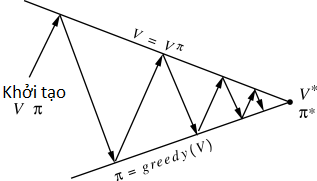
\includegraphics[width=.8\textwidth]{policy_iteration}
	\caption[Hội tụ của quy trình tìm kiếm chính sách tối ưu]{Hình minh họa quá trình hội tụ của quy trình lặp chính sách.
	Ta có một chính sách $\pi$, đầu tiên ta thực hiện đánh giá chính sách $\pi$ để có được hàm giá trị theo chính sách này. 
	Khi có được hàm giá trị, ta thực hiện cải thiện chính sách bằng kỹ thuật tham lam. 
	Sau khi có được chính sách mới, ta tiếp tục đánh giá chính sách để có được hàm giá trị của chính sách đó. 
	Quá trình này được lặp nhiều lần cho đến khi ta đạt được chính sách tối ưu và hàm giá trị tối ưu.}
	\label{fig:policy_iteration_MDP}	
\end{figure}

\subsection{Phương pháp lặp giá trị}
Một nhược điểm của phương pháp lặp chính sách nằm ở giai đoạn đánh giá chính sách của phương pháp này. Bản thân giai đoạn này cũng là một quá trình lặp để tìm ra hàm giá trị của chính sách $\pi$ đang theo. Ngoài ra, giai đoạn này cũng đã được chứng minh sẽ tìm được chính xác hàm giá trị $v_{\pi}$ khi lặp vô hạn lần. Câu hỏi đặt ra là: Để tìm chính sách tối ưu, chúng ta có cần phải xác định chính xác hàm giá trị $v_{\pi}$ của chính sách $\pi$ hiện tại hay không? \cite{smallwood1973optimal} đã đề xuất một phương pháp có thể tìm đươc chính sách tối ưu mà không cần xác định hàm giá trị $v_{\pi}$, được gọi là phương pháp lặp giá trị. Trong phương pháp lặp chính sách, tại mỗi vòng lặp một ước lượng $V$ cho hàm giá trị $v_{\pi}$ được cập nhật nhiều lần để đạt chính xác hàm $v_{\pi}$ trước khi thực hiện cải thiện chính sách. Ngược lại, phương pháp lặp giá trị thực hiện duy nhất một lần cập nhật ước lượng kết hợp với tối ưu bằng toán tử $\max$ ngay trong mỗi vòng lặp của nó. Chính vì vậy mà phương pháp lặp giá trị không tách biệt hai giai đoạn rõ ràng như phương pháp lặp chính sách và mục tiêu của phương pháp này là tìm được hàm giá trị tối ưu $v_*$. Phương trình \ref{eq:val_iteration} mô tả cách thức cập nhật hàm giá trị cũng như tối ưu trong một lần lặp. Ý nghĩa của phương trình này là dùng giá trị hành động lớn nhất cập nhật giá trị cho một trạng thái $s$.
\begin{align}
	v_{k+1}(s) = {} & \max_{a}\mathbb{E}\left[\mathit{R}_{t+1} + \gamma v_{k}(\mathit{S}_{t+1}) \mid \mathit{S}_{t} = s, \mathit{A}_t = a\right] \notag \\
	= {} & \max_{a}\sum_{s' \in \mathcal{S}}\mathcal{P}_{ss'}^{a}\left[\mathit{R}_{t+1} + \gamma v_{k}(s')\right] \label{eq:val_iteration}
\end{align}
với $s \in \mathcal{S}$ và $v_{0}$ được khởi tạo ngẫu nhiên. Qua nhiều cập nhật chuỗi $\{v_{k}\}$ sẽ hội tụ về hàm giá trị tối ưu $v_*$.

Cách thức cập nhật của phương pháp lặp giá trị dựa trên phương trình Bellman của hàm giá trị trạng thái tối ưu \ref{eq:bellman_optimal_state}. Mô hình cập nhật của phương pháp lặp giá trị tương tự mô hình cập nhật của phương pháp lặp chính sách \ref{fig:Update_Value_DP} ngoại trừ nó yêu cầu giá trị cực đại (maximum) được chọn qua các hành động. Thêm vào đó quá trình cập nhật của lặp chính sách để tính hàm giá trị trạng thái $v_{\pi}$ của chính sách $\pi$ hiện tại, trong khi đó quá trình cập nhật của lặp giá trị để tính hàm giá trị trạng thái tối ưu $v_*$. Các bước thực hiện trong phương pháp lặp giá trị được mô tả trong thuật toán \ref{alg_val_iteration}.
\begin{algorithm}
	\newalgname{Thuật toán}
	\caption{Phương pháp lặp giá trị trên hàm giá trị trạng thái}
	\label{alg_val_iteration}
	\begin{algorithmic}[1]
		\renewcommand{\algorithmicrequire}{\textbf{Đầu vào:}}
		\renewcommand{\algorithmicensure}{\textbf{Đầu ra:}}
		\algnewcommand\algorithmicoperation{\textbf{Thao tác:}}
		\algnewcommand\Operation{\item[\algorithmicoperation]}
		
		\Require
		\Ensure Hàm giá trị $V$ xấp xỉ hàm giá trị tối ưu $v_{*}$
		
		\Operation
		\State Khởi tạo ngẫu nhiên $V(s)$ cho tất cả trạng thái $s$ không phải trạng thái kết thúc. Nếu $s$ là trạng thái kết thúc, $V(s) = 0$
		\Repeat
		\State $\Delta \leftarrow 0$ \%\% Tính độ khác biệt giữa hàm giá trị cũ và giá trị mới. Độ lớn của $\Delta$ được xác định là độ khác biệt lớn nhất giữa giá trị cũ và giá trị mới của một trạng thái trong tất cả các trạng thái.
		\For{$s \in \mathcal{S}$} \%\% Với mỗi trạng thái
		\State $v \leftarrow V(s)$ \%\% Lưu giá trị hiện tại của trạng thái $s$
		\State $V(s) \leftarrow \max_{a}\sum_{s' \in \mathcal{S}}\mathcal{P}_{ss'}^{a}\left[\mathcal{R}_{s}^{a} + \gamma V(s')\right]$ \%\% Duyệt và chọn ra giá trị hành động lớn nhất làm giá trị mới của trạng thái $s$
		\State $\Delta \leftarrow \max(\Delta,|v - V(s)|)$
		\EndFor
		\Until $\Delta < \theta$ (Một lượng đủ nhỏ)
	\end{algorithmic}
\end{algorithm}

\textbf{Ví dụ: Bài toán di chuyển trên lưới $4 \times 4$} Hệ thống có thể thực hiện 4 hành động: lên, xuống, qua trái, qua phải. Vị trí đích là góc trái trên của lưới. Hệ thống sẽ dừng nếu di chuyển ra ngoài lưới. Mỗi hành động của hệ thống đều nhận được kiểm thưởng là -1. Và nhận được điểm thưởng +7 khi hệ thống về đích. Mục tiêu của hệ thống là tìm được đường về vị trí đích.
Giả sử có nhiễu trong quá trình hệ thống di chuyển: 70\% hệ thống sẽ di chuyển theo hướng trùng với hành động đã thực hiện, 30\% hệ thống sẽ di chuyển khác hướng với hành động thực hiện. Ví dụ nếu hệ thống thực hiện hành động đi lên thì 70\% hệ thống sẽ di chuyển đi lên, 10\% hệ thống di chuyển sang trái, 10\% hệ thống di chuyển sang phải, và 10\% hệ thống di chuyển xuống dưới. Hệ số $\gamma = 1$. Hình \ref{grid_problem} minh họa bài toán này.
\begin{figure}
	\centering
	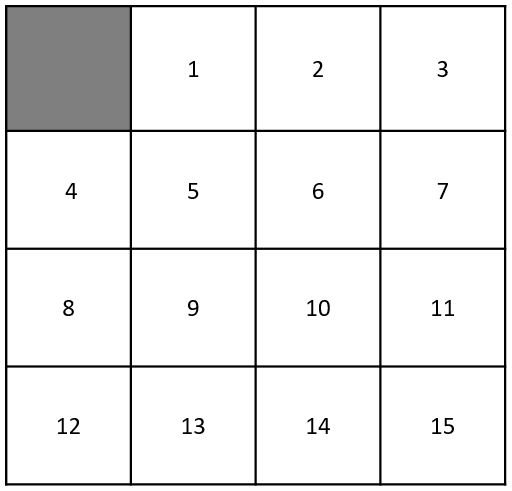
\includegraphics[width=60mm, height =60mm]{baitoan}
	\caption[Bài toán di chuyển trên lưới]{Bài toán di chuyển trên lưới}
	\label{grid_problem}
\end{figure}

Qua ví dụ \ref{fig:VI_process} minh họa quá trình tìm hàm giá trị trạng thái tối ưu bằng quá trình lặp giá trị, ta có thể thấy hàm giá trị trạng thái dần hội tụ về hàm giá trị $q_*$ thông qua những chính sách tương ứng của mỗi lần cập nhật.
\begin{figure*}[t!]
	\centering
	\begin{tabular}{c}
		\begin{subfigure}[t]{0.5\textwidth}
			\centering
			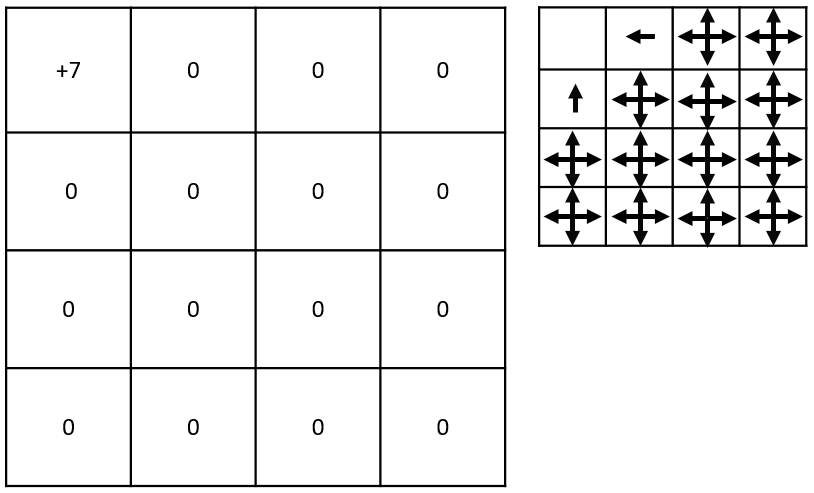
\includegraphics[height=45mm]{step_1}
			\caption{Khởi tạo hàm giá trị $V$}
		\end{subfigure}%
		~ 
		\begin{subfigure}[t]{0.5\textwidth}
			\centering
			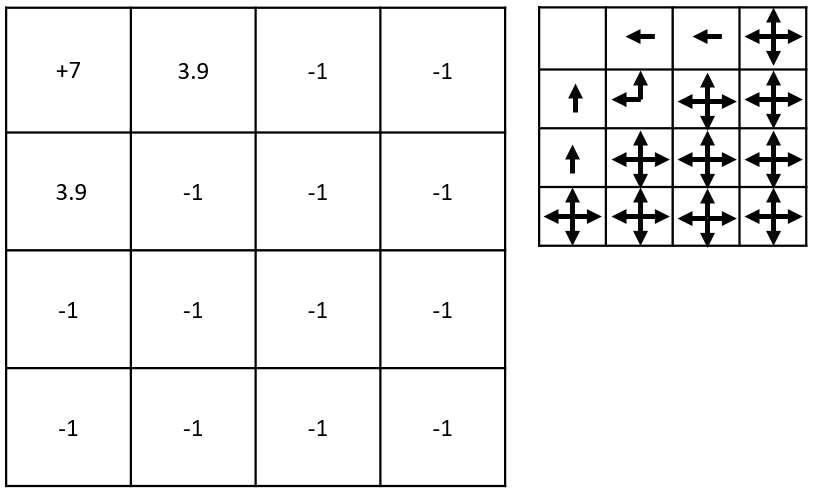
\includegraphics[height=45mm]{step_2}
			\caption{Cập nhật hàm giá trị lần 1, và chính sách tham lam trên hàm giá trị hiện tại}
		\end{subfigure} \\~\\
		\begin{subfigure}[t]{0.5\textwidth}
			\centering
			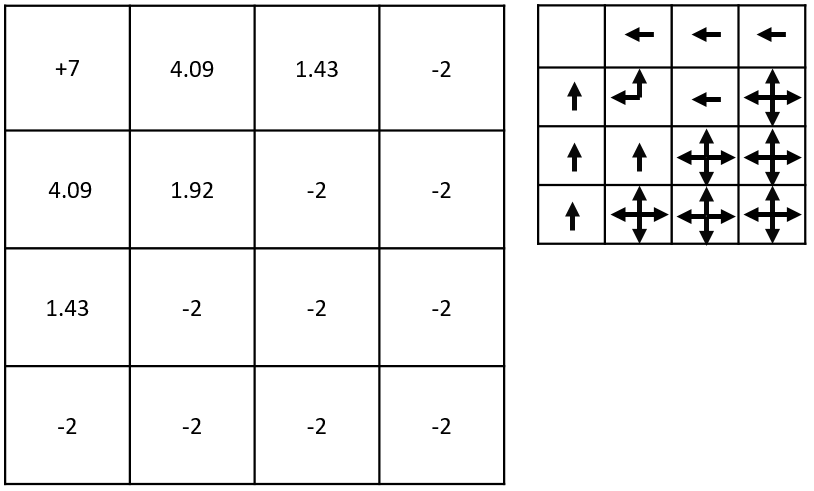
\includegraphics[height=45mm]{step_3}
			\caption{Cập nhật hàm giá trị lần 2, và chính sách tham lam trên hàm giá trị hiện tại}
		\end{subfigure}%
		~ 
		\begin{subfigure}[t]{0.5\textwidth}
			\centering
			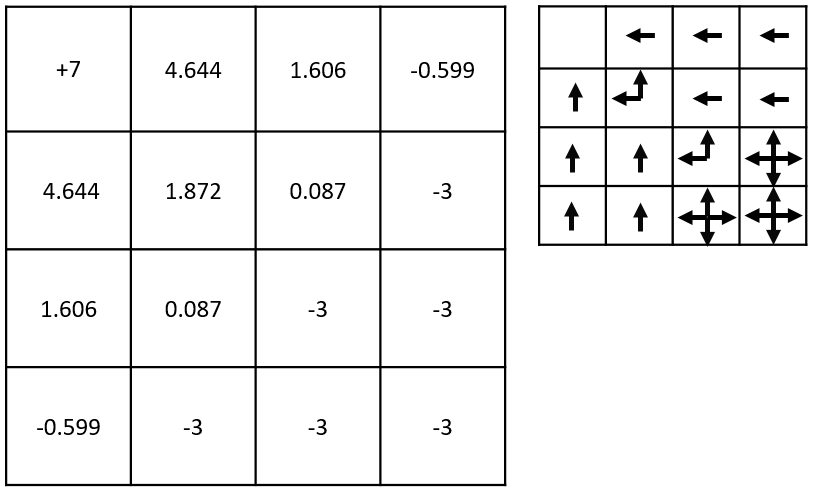
\includegraphics[height=45mm]{step_4}
			\caption{Cập nhật hàm giá trị lần 3, và chính sách tham lam trên hàm giá trị hiện tại}
		\end{subfigure} \\~\\
		\begin{subfigure}[t]{0.5\textwidth}
			\centering
			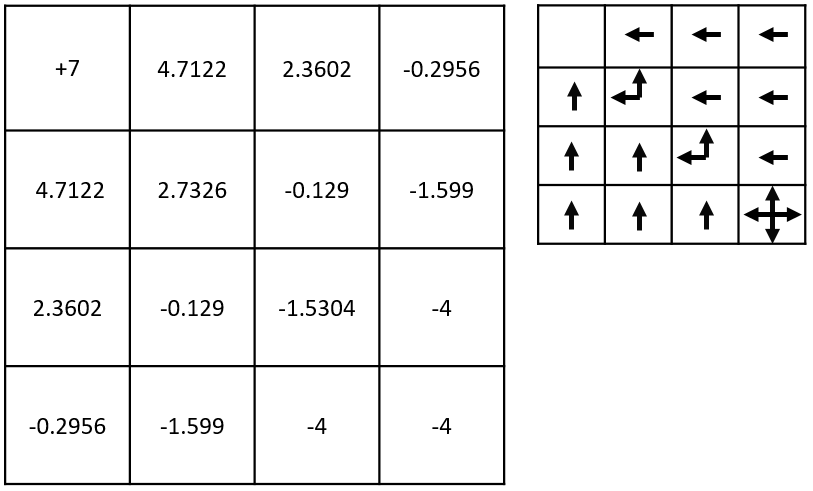
\includegraphics[height=45mm]{step_5}
			\caption{Cập nhật hàm giá trị lần 4, và chính sách tham lam trên hàm giá trị hiện tại}
		\end{subfigure}%
		~ 
		\begin{subfigure}[t]{0.5\textwidth}
			\centering
			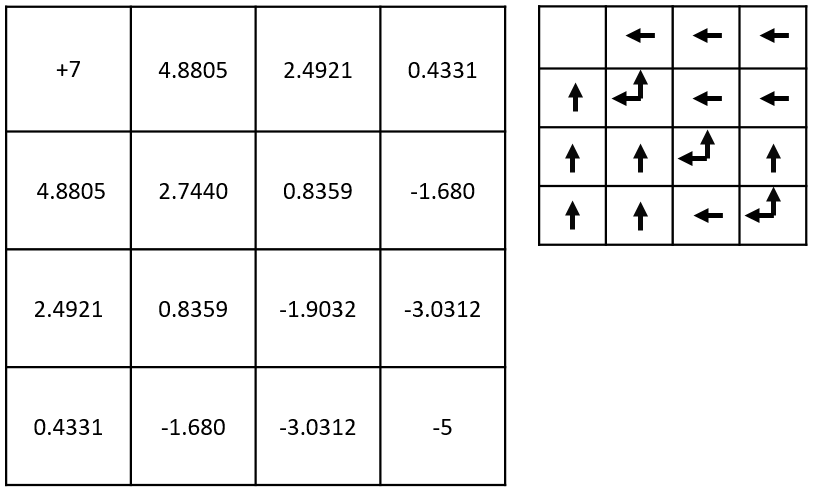
\includegraphics[height=45mm]{step_6}
			\caption{Cập nhật hàm giá trị lần 5, và chính sách tham lam trên hàm giá trị hiện tại}
		\end{subfigure}
	\end{tabular}
	\caption[Minh họa quy trình lặp giá trị]{Quy trình cập nhật hàm giá trị trạng thái bằng phương pháp lặp giá trị}
	\label{fig:VI_process}
\end{figure*}

Trong nhiều trường hợp việc sử dụng hàm giá trị hành động trở nên khả thi hơn hàm giá trị trạng thái. Thực vậy, với việc có được mô hình MDP của môi trường , hàm giá trị trạng thái là đủ để xác định chính sách tối ưu nhưng việc xác định này phải qua một bước trung gian thông qua ma trận chuyển trạng thái. Nói cách khác để xác định chính sách tối ưu trên hàm giá trị trạng thái, hệ thống phải xác định những trạng thái tiếp theo có thể đến thông qua ma trận chuyển trạng thái, sau đó chọn hành động mà giúp cho hệ thống có thể đến được trạng thái tiếp theo có giá trị lớn nhất. Tuy nhiên trong một số bài toán hệ thống không biết mô hình MDP của môi trường thì hàm giá trị trạng thái là không đủ để xác định chính sách tối ưu. Ngược lại, có được hàm giá trị hành động là đủ để xác định chính sách tối ưu trong cả hai trường hợp biết và không biết MDP. Mặc dù khi biết được mô hình MDP của môi trường, việc xác định chính sách tối ưu bằng hàm giá trị hành động được cho là tốn kém trong việc lưu trữ nhưng những phương pháp tìm chính sách tối ưu vẫn thường sử dụng loại hàm giá trị này do nó có thể sử dụng trong cả hai trường hợp. Trong phương pháp lặp giá trị, ta cũng có thể xác định hàm giá trị hành động tối ưu qua nhiều lần lặp. Phương trình \ref{eq:q_val_iteration} minh họa cách thức cập nhật ước lượng của hàm giá trị $q_*$
\begin{align}
q_{k+1}(s,a) = {} & \mathbb{E}\left[\mathit{R}_{t+1} + \gamma \max_{a'}q_{k}(\mathit{S}_{t+1},a') \mid \mathit{S}_{t} = s, \mathit{A}_t = a\right] \notag \\
= {} & \sum_{s' \in \mathcal{S}}\mathcal{P}_{ss'}^{a}\left[\mathit{R}_{t+1} + \gamma \max_{a'}q_{k}(s',a')\right] \label{eq:q_val_iteration}
\end{align}
với $s \in \mathcal{S}, a \in \mathcal{A}(s)$. Thuật toán \ref{alg_qval_iteration} minh họa các bước thực hiện lặp giá trị cho hàm hành động.

\begin{algorithm}
	\newalgname{Thuật toán}
	\caption{Phương pháp lặp giá trị trên hàm giá trị hành động}
	\label{alg_qval_iteration}
	\begin{algorithmic}[1]
		\renewcommand{\algorithmicrequire}{\textbf{Đầu vào:}}
		\renewcommand{\algorithmicensure}{\textbf{Đầu ra:}}
		\algnewcommand\algorithmicoperation{\textbf{Thao tác:}}
		\algnewcommand\Operation{\item[\algorithmicoperation]}
		
		\Require
		\Ensure Hàm giá trị $Q$ xấp xỉ hàm giá trị tối ưu $q_{*}$
		
		\Operation
		\State Khởi tạo ngẫu nhiên $Q(s,a)$ cho tất cả các cặp trạng thái $s$ và hành động $a$ với $s$ không phải trạng thái kết thúc. Nếu $s$ là trạng thái kết thúc, $Q(s,a) = 0$
		\Repeat
		\State $\Delta \leftarrow 0$ \%\% Tính độ khác biệt giữa hàm giá trị cũ và giá trị mới. Độ lớn của $\Delta$ được xác định là độ khác biệt lớn nhất giữa giá trị cũ và giá trị mới của một trạng thái trong tất cả các trạng thái.
		\For{$s \in \mathcal{S}$} \%\% Với mỗi trạng thái
		\State $q \leftarrow Q(s,a)$ \%\% Lưu giá trị hiện tại của cặp trạng thái, hành động $(s,a)$
		\State $Q(s,a) \leftarrow \sum_{s' \in \mathcal{S}}\mathcal{P}_{ss'}^{a}\left[\mathcal{R}_{s}^{a} + \gamma \max_{a'}Q(s',a')\right]$ \%\% Thực hiện cập nhật
		\State $\Delta \leftarrow \max(\Delta,|q - Q(s,a)|)$
		\EndFor
		\Until $\Delta < \theta$ (Một lượng đủ nhỏ)
	\end{algorithmic}
\end{algorithm}


%\section{Tìm chính sách tối ưu bằng phương pháp lặp chính sách trong bài toán thực tế}
%Trong nhiều bài toán thực tế thông thường chúng ta không có kiến thức đầy đủ về môi trường như ma trận chuyển trạng thái $\mathcal{P}$, ma trận điểm thưởng $\mathcal{R}$, tập các trạng thái $\mathcal{A}$. Do đó một yêu cầu được đặt ra là hệ thống phải có khả năng học từ những thông tin mà nó tiếp nhận được qua việc tương tác với môi trường. Các thông tin này thường ở dạng chuỗi (trạng thái, hành động, điểm thưởng)
%$\mathit{S}_1, \mathit{A}_1, \mathit{R}_2, \mathit{S}_2, \mathit{A}_2, \mathit{R}_3, \dots, \mathit{S}_T$. Với $T$ là thời điểm kết thúc việc tương tác của hệ thống với môi trường.
%
%\subsection{Phương pháp đánh giá chính sách}
%Trong phần này, chúng em sẽ trình bày một số phương pháp được áp dụng để đánh giá chính sách.
%
%\subsubsection{Phương pháp Monte Carlo (MC)}
%Tương tự với quy hoạch động, Monte Carlo (MC) xác định hàm giá trị của một chính sách bằng cách cập nhật hàm giá trị khởi tạo qua nhiều vòng lặp. Điểm biệt khác với quy hoạch động của phương pháp MC là nó có thể áp dụng để đánh giá chính sách khi hệ thông không có kiến thức đầy đủ về môi trường. MC dựa trên những thông tin mà hệ thông có được qua việc tương tác với môi trường để xấp xỉ hàm giá trị. Thông thường những thông tin này được chia thành các \textit{mẫu thực nghiệm}. Mỗi mẫu thực nghiệm là một chuỗi bắt đầu từ một trạng thái bất kỳ cho đến khi đạt được một trong những trạng thái kết thúc. Khi đó MC chỉ thực hiện cập nhật hàm giá trị khi kết thúc một mẫu thực nghiệm.
%
%Ý tưởng của MC là xác định giá trị của một trạng thái $s$ qua các mẫu thực nghiệm có sự xuất hiện trạng thái đó. Phương pháp MC xác định giá trị của trạng thái $s$ bằng cách trung bình các tổng điểm thưởng mà hệ thông nhận được sau khi quan sát được trạng thái $s$. Khi quan sát càng nhiều mẫu thực nghiệm có trạng thái $s$ xuất hiện, giá trị trung bình sẽ càng xấp xỉ tốt giá trị thực của trạng thái này theo chính sách $\pi$.
%
%Một mẫu thực nghiệm là những thông tin có được trong quá trình hệ thống tương tác với môi trường bằng chính sách $\pi$. Giá trị của trạng thái $s$, $v(s)$, được tính dựa trên những mẫu thực nghiệm có trạng thái $s$ xuất hiện. Một trạng thái $s$ có thể xuất hiện nhiều lần trong một mẫu thực nghiệm. Lần xuất hiện đầu tiên của trạng thái $s$ trong một mẫu thực nghiệm được gọi là first-visit trạng thái đó. Phương pháp first-visit MC xác định giá trị trạng thái $s$, $v_{\pi}(s)$, bằng trung bình tất cả các tổng điểm thưởng mà hệ thống nhận sau lần first-visit của trạng thái $s$ trong các mẫu thực nghiệm. Tổng thể của việc đánh giá chính sách bằng first-visit MC được trình bày ở thuật toán \ref{alg_MC}. Hình \ref{fig:first_visit_MC} minh họa cách thức cập nhật hàm giá trị trên một mẫu thực nghiệm.
%\begin{algorithm}
%	\newalgname{Thuật toán}
%	\caption{Xác định hàm giá trị trạng thái bằng phương pháp first-visit MC}
%	\label{alg_MC}
%	\begin{algorithmic}[1]
%		\renewcommand{\algorithmicrequire}{\textbf{Đầu vào:}}
%		\renewcommand{\algorithmicensure}{\textbf{Đầu ra:}}
%		\algnewcommand\algorithmicoperation{\textbf{Thao tác:}}
%		\algnewcommand\Operation{\item[\algorithmicoperation]}
%		
%		\Require Chính sách $\pi$ cần đánh giá
%		\Ensure Hàm giá trị $V$ xấp xỉ hàm giá trị $v_{\pi}$ của chính sách $\pi$
%		
%		\Operation
%		\State Khởi tạo ngẫu nhiên $V(s)$ cho tất cả trạng thái $s$ không phải trạng thái kết thúc. Nếu $s$ là trạng thái kết thúc, $V(s) = 0$
%		\State Khởi tạo danh sách rỗng \textbf{Returns($s$)} cho tất cả trạng thái $s \in \mathcal{S}$ \%\% Danh sách Returns($s$) chứa tất cả các tổng điểm thưởng mà hệ thống nhận được sau lần first-visit của trạng thái $s$ trong các mẫu thực nghiệm.
%		\Repeat
%		\State Tạo một mẫu thực nghiệm $E$ bằng chính sách $\pi$
%		\For{mỗi trạng thái $s$ xuất hiện lần đầu trong $E$}
%		\State $G \leftarrow$ tổng điểm thưởng nhận được sau lần xuất hiện đầu tiên của $s$
%		\State Thêm $G$ vào danh sách Returns(s)
%		\State $V(s) \leftarrow$ average(Returns(s))
%		\EndFor
%		\Until Thỏa điều kiện dừng
%	\end{algorithmic}
%\end{algorithm}
%\begin{figure}
%	\centering
%	\begin{tikzpicture}[node distance=4.5cm,>=stealth',bend angle=45,auto]
%	
%	\tikzstyle{state}=[circle,thick,draw=blue!75,fill=white!20,minimum size = 10mm, inner sep=0pt]
%	\tikzstyle{action}=[circle,draw=black!75,
%	fill=black!75,minimum size=2mm]
%	\tikzstyle{terminal}=[square,draw=black!60,
%	fill=black!75,minimum size=10mm]
%	
%	
%	\tikzstyle{every label}=[red]
%	
%	\begin{scope}
%	% First net
%	\node [state, label={[name=label node]below:$\mathit{S}_0$}] (s1)                           {};
%	
%	\node [action] (a1) [right = 0.7cm of s1]{}
%	edge (s1);
%	
%	\node[state, fill=green, label={[name=label node]below:$\mathit{S}_1$}] (s2)  [right = 0.7cm of a1]{}
%	edge node[above]{$r_1$} (a1);
%	
%	\node [action] (a2) [right = 0.7cm of s2]{}
%	edge (s2);
%	
%	\node[state, fill=red, label={[name=label node]below:$\mathit{S}_2$}] (s3)  [right = 0.7cm of a2]{}
%	edge node[above]{$r_2$} (a2);
%	
%	\node [action] (a3) [right = 0.7cm of s3]{}
%	edge (s3);
%	
%	\node (etc) [right = 0.7cm of a3] {\large $\dots$};
%	
%	\node [state, fill=green, label={[name=label node]below:$\mathit{S}_{T-1}$}] (s4) [right = 0.7cm of etc]{};
%	
%	\node [action] (a4) [right = 0.7cm of s4]{}
%	edge (s4);
%	
%	\node [state, fill = gray, label={[name=label node]below:Trạng thái kết thúc}] (t) [right = 0.7cm of a4]{}
%	edge node[above]{$r_{T}$} (a4)
%	edge [post,bend right] (s3)
%	edge [post,bend right] (s2)
%	edge [post,bend right] node[above]{Cập nhật giá trị} (s1);
%	
%	\end{scope}	
%	\end{tikzpicture}
%	\caption[Cập nhật hàm giá trị bằng phương pháp Monte Carlo]{Đồ thị minh họa cập nhật hàm giá trị trên một mẫu thực nghiệm bằng phương pháp first-visit MC. Hình tròn lớn ký hiệu cho trạng thái xuất hiện. Hình tròn nhỏ ký hiệu cho hành động thực hiện. Màu xác khác nhau giữa các hình tròn biểu thị cho sự khác nhau giữa các trạng thái. Phương pháp first-visit MC chỉ cập nhật giá trị cho các trạng thái khi kết thúc một mẫu thực nghiệm, và mỗi trạng thái chỉ được cập nhật một lần mặc dù trạng thái đó có thể xuất hiện nhiều lần trong cùng một mẫu.}
%	\label{fig:first_visit_MC}
%\end{figure}
%
%Trong nhiều trường hợp, hệ thống không có được mô hình của môi trường, việc sử dụng hàm giá trị hành động trở nên khả thi hơn hàm giá trị trạng thái. Với việc có được mô hình của môi trường, hàm giá trị trạng thái là đủ để cải thiện một chính xách trở nên tốt hơn; nó đơn giản là nhìn trước trạng thái tiếp theo có thể đến và chọn bất kỳ hành động nào dẫn đến trạng thái đó mà đạt được nhiều điểm thưởng nhất. Ngược lại, nếu không có được mô hình của môi trường, hàm giá trị trạng thái là không đủ do hệ thống không thể xác định được trạng thái tiếp theo là trạng thái gì. Vì vậy, nó cần đánh giá giá trị của mỗi hành động trong mỗi trạng thái để xác định hành động nào nên thực hiện ở mỗi trạng thái qua đó cải thiện chính sách đang thực hiện.
%Việc xác định hàm giá trị hành động $q_{\pi}$ được thực hiện tương tự như đã làm với hàm giá trị trạng thái $v_{\pi}$. Để xác định giá trị của hành động $a$ tại trạng thái $s$, nó thực hiện tính trung bình các tổng điểm thưởng mà hệ thộng nhận được dựa vào các mẫu thực nghiệm có sự xuất hiện của cặp trạng thái, hành động $(s,a)$. Lần xuất hiện đầu tiên của cặp trạng thái và hành động $(s,a)$ trong một mẫu thực nghiệm được gọi là first-visit của cặp trạng thái và hành động đó. Phương pháp first-visit MC xác định giá trị của hành động $a$ ở trạng thái $s$, $q_{\pi}(s,a)$, bằng trung bình tất cả các tổng điểm thưởng nhận được sau lần first-visit của cặp $(s,a)$ trong các mẫu thực nghiệm. Thuật toán \ref{alg_MC_action} trình bày cách thức xác định hàm giá trị hành động bằng first-visit MC.
%\begin{algorithm}
%	\newalgname{Thuật toán}
%	\caption{Xác định hàm giá trị hành động bằng phương pháp first-visit MC}
%	\label{alg_MC_action}
%	\begin{algorithmic}[1]
%		\renewcommand{\algorithmicrequire}{\textbf{Đầu vào:}}
%		\renewcommand{\algorithmicensure}{\textbf{Đầu ra:}}
%		\algnewcommand\algorithmicoperation{\textbf{Thao tác:}}
%		\algnewcommand\Operation{\item[\algorithmicoperation]}
%		
%		\Require Chính sách $\pi$ cần đánh giá
%		\Ensure Hàm giá trị $V$ xấp xỉ hàm giá trị $v_{\pi}$ của chính sách $\pi$
%		
%		\Operation
%		\State Khởi tạo ngẫu nhiên $Q(s,a)$ cho tất cả các cặp trạng thái, hành động $s,a$.
%		\State Khởi tạo danh sách rỗng \textbf{Returns($s,a$)} cho tất cả các cặp trạng thái, hành động ($s,a$). \%\% Danh sách Returns($s,a$) chứa tất cả các tổng điểm thưởng mà hệ thống nhận được sau lần first-visit của cặp trạng thái, hành động ($s,a$) trong các mẫu thực nghiệm.
%		\Repeat
%		\State Tạo một thực nghiệm $E$ bằng chính sách $\pi$
%		\For{mỗi cặp trạng thái, hành động $(s,a)$ xuất hiện lần đầu trong $E$}
%		\State $G \leftarrow$ tổng điểm thưởng nhận được sau lần xuất hiện đầu tiên của cặp trạng thái, hành động $(s,a)$
%		\State Thêm $G$ vào danh sách Returns($s,a$)
%		\State $Q(s,a) \leftarrow$ average(Returns($s$))
%		\EndFor
%		\Until Thỏa điều kiện dừng
%	\end{algorithmic}
%\end{algorithm}
%
%\subsubsection{Phương pháp Temporal Difference (TD)}
%Phương pháp Temporal Difference (TD) kết hợp ý tưởng giữa Monte Carlo và quy hoạch động. Giống như Monte Carlo, phương pháp TD có thể học trực tiếp từ các mẫu thực nghiệm có được qua việc tương tác của hệ thống với môi trường mà không cần có mô hình của môi trường. Mặt khác tương tự với quy hoạch động, phương pháp TD thựa hiện cập nhật giá trị dựa trên những phần đã được xác định trước đó mà không phải đợi đến khi kết thúc một mẫu thực nghiệm như MC.
%
%Giả sử ta có các trung bình $\mu_{1}$, $\mu_{2}$, ... của chuỗi $x_1, x_2, ...$ có thể được tính như sau:
%\begin{align}
%\mu_{k} = {}& \frac{1}{k}\sum_{j=1}^{k}x_{j} \notag \\
%= {}& \frac{1}{k} \left(x_k + \sum_{j = 1}^{k - 1}x_j\right) \notag \\
%= {}& \frac{1}{k}(x_k + \left(k - 1\right)\mu_{k-1}) \notag \\
%= {}& \mu_{k - 1} + \frac{1}{k}(x_k - \mu_{k-1}) \label{eq:mean}
%\end{align}
%Phương pháp Monte Carlo phải đợi cho đến khi xác định được tổng điểm tưởng sau lần xuất hiện của một trạng thái để thực hiện cập nhật giá trị cho trạng thái đó, và giá trị của một trạng thái được cập nhật qua nhiều vòng lặp. Dựa vào phương trình \ref{eq:mean} giá trị của mỗi trạng thái có thể được cập nhật như sau:
%\begin{align}
%N(\mathit{S}_{t}) & \leftarrow N(\mathit{S}_{t}) + 1 \\
%V(\mathit{S}_t) & \leftarrow V(\mathit{S}_t) + \frac{1}{N(\mathit{S}_{t})}(\mathit{G_t} - V(\mathit{S}_t)) \label{eq:update_value_MC}
%\end{align}
%Khi đó $\mathit{G}_t$ được gọi là mục tiêu cập nhật cho $V(S_t)$. Mặt khác, khi môi trường không ổn định việc cập nhật giá trị trạng thái theo \ref{eq:update_value_MC}  thường được cố định bằng hệ số $\alpha$:
%\begin{equation}
%V(\mathit{S}_t) \leftarrow V(\mathit{S}_t) + \alpha(\mathit{G_t} - V(\mathit{S}_t))
%\end{equation}
%Khác với phương pháp MC, phương pháp TD chỉ cần đợi tới bước tiếp theo ngay sau đó $t+1$ để hình thành một cái đích cho việc cập nhật qua việc quan sát điểm thưởng $R_{t+1}$ và giá trị của trạng thái tiếp theo $V(\mathit{S}_{t+1})$. Phương pháp TD đơn giản nhất được gọi là TD(0). Cách thức cập nhật giá trị của một trạng thái trong phương pháp này như sau:
%\begin{equation}
%V(\mathit{S}_t) \leftarrow 	V(\mathit{S}_t) + \alpha[\mathit{R}_{t+1} + \gamma V(\mathit{S}_{t+1}) - V(\mathit{S}_t)]
%\label{eq:update_value_TD}
%\end{equation}
%Trong \ref{eq:update_value_TD} ta thấy mục tiêu cập nhật cho $V(\mathit{S}_t)$ trong TD(0) là $\mathit{R}_{t+1} + \gamma V(\mathit{S}_{t+1})$. Vì phương pháp TD thực hiện cập nhật giá trị của một trạng thái dựa một phần vào các giá trị của những trạng thái tiếp theo nên phương pháp này là một phương pháp "bootstapping", tương tự với quy hoạch động. Như đã định nghĩa trong \ref{sec:policy_value}, giá trị của trạng thái $s$ dưới chính sách $\pi$ được xác định:
%\begin{align}
%v_{\pi}(s) = {} & \mathbb{E}_{\pi}\left [\mathit{G}_t \mid \mathit{S}_{t} = s\right ] \label{eq:value_base_return} \\
%={} & \mathbb{E}_{\pi}\left [\sum_{k = 0}^{\infty}\gamma^{k}\mathit{R}_{t+k+1} \middle|\ \mathit{S}_t= s\right ] \notag \\
%= {} & \mathbb{E}_{\pi}\left [\mathit{R}_{t+1} + \gamma \sum_{k = 0}^{\infty}\gamma^{k}\mathit{R}_{t+k+2} \middle|\ \mathit{S}_t= s\right ] \notag \\
%= {} & \mathbb{E}_{\pi} \left[\mathit{R}_{t+1} + \gamma v_{\pi}(\mathit{S}_{t+1}) \mid \mathit{S}_t = s\right] \label{eq:value_base_bootstrap}
%\end{align}
%Qua đó, ta thấy rằng phương pháp MC sử dụng ước lượng của \ref{eq:value_base_return} là mục tiêu cập nhật; trong khi đó phương pháp quy hoạch động sử dụng ước lượng của \ref{eq:value_base_bootstrap}. Mục tiêu cập nhật của MC là một ước lượng vì không biết giá trị kỳ vọng trong \ref{eq:value_base_return} do đó tổng điểm thưởng trên một mẫu được sử dụng để thay thế cho giá trị kỳ vọng thực sự của nó. Mục tiêu cập nhật của quy hoạch động cũng là một ước lượng không phải vì giá trị kỳ vọng do trong quy hoạch động chúng ta đã giả định hệ thống có mô hình của môi trường; nhưng là vì $v_{\pi}(\mathit{S}_{t+1})$ là không biết do hiện tại nó đang được đánh giá; do đó $V(\mathit{S}_{t+1})$ được sử dụng để thay thế. Mục tiêu cập nhất trong TD là một ước lượng do cả hai nguyên nhân trên nên TD ước lượng giá trị kỳ vọng trong \ref{eq:value_base_return} qua mẫu và sử dụng ước lượng của hàm giá trị hiện tại $V$ để thay thế cho hàm giá trị đúng $v_{\pi}$. Vì vậy, phương pháp TD được cho là phương pháp kết hợp cách lấy mẫu của MC và bootstrapping của quy hoạch động. Từng bước thực hiện cập nhật hàm giá trị bằng phương pháp TD(0) được trình bày trong thuật toán thuật toán \ref{alg_TD_Zero}.
%\begin{algorithm}
%	\newalgname{Thuật toán}
%	\caption{Xác định hàm giá trị trạng thái bằng TD(0)}
%	\label{alg_TD_Zero}
%	\begin{algorithmic}[1]
%		\renewcommand{\algorithmicrequire}{\textbf{Đầu vào:}}
%		\renewcommand{\algorithmicensure}{\textbf{Đầu ra:}}
%		\algnewcommand\algorithmicoperation{\textbf{Thao tác:}}
%		\algnewcommand\Operation{\item[\algorithmicoperation]}
%		
%		\Require Chính sách $\pi$ cần đánh giá
%		\Ensure Hàm giá trị $V$ xấp xỉ hàm giá trị $v_{\pi}$ của chính sách $\pi$
%		
%		\Operation
%		\Repeat
%		\State Tạo một mẫu thực nghiệm $E$ bằng chính sách $\pi$
%		\State Khởi tạo trạng thái $s$
%		\For{mỗi bước trong $E$}
%		\State $A \leftarrow$ hành động được chọn theo chính $\pi$ tại $s$
%		\State Thực hiện hành động $A$; quan sát điểm thưởng $r$ nhận được, và trạng thái tiếp theo $s'$
%		\State $V(s) \leftarrow V(s) + \alpha \left[r + \gamma V(s') - V(s)\right]$ \%\% Thực hiện cập nhật giá trị cho trạng thái $s$
%		\State $s \leftarrow s'$
%		\EndFor
%		\Until thỏa điều kiện dừng
%	\end{algorithmic}
%\end{algorithm}
%
%Với bất kỳ chính sách $\pi$ cố định. Việc xác định hàm giá trị bằng phương pháp TD đã được chứng minh hội tu về hàm giá trị $v_{\pi}$ theo luật số lớn. Trong thực nghiệm, phương pháp TD thường hội tụ về hàm giá trị $v_{\pi}$ nhanh hơn phương pháp MC.
%
%Phương pháp TD(0) xem giá trị của các trạng thái kế tiếp từ một trạng thái $s$ là giá trị đại diện cho lượng điểm thưởng mà trạng thái $s$ có thể nhận được ở tương lai; và dựa vào giá trị đại diện này và điểm thưởng nhận được ngay trạng thái $s$ để xác định giá trị của trạng thái đó. Tổng quát cho phương pháp TD là n-step TD. Để xác định giá trị của một trạng thái $s$, phương pháp n-step TD xem giá trị của trạng thái thứ $n$ sau đó là giá trị đại diện cho lượng điểm thưởng mà hệ thống có thể nhận được từ bước thứ $n$ trở về sau; và xác định giá trị của trạng thái $s$ dựa trên giá trị đại diện này cùng với điểm thưởng đã nhận được ở $n$ bước sáu đó. Hình \ref{fig:n_TD} minh họa cách xác định hàm giá trị trạng thái bằng phương pháp $n$-step TD. Phương pháp này thực hiện cập nhật cho một trạng thái ở bước thứ $n$ sau khi trạng thái $s$ xuất hiện trong mẫu thực nghiệm. 
%\begin{figure}
%	\centering
%	\begin{tikzpicture}[>=stealth,bend angle=45,auto]
%	
%	\tikzstyle{state}=[circle,thick,draw=blue!75,fill=white!20,minimum size = 5mm, inner sep=0pt]
%	\tikzstyle{action}=[circle,draw=black!75,
%	fill=black!75,minimum size=2mm]
%	
%	\tikzstyle{every label}=[red]
%	
%	\begin{scope}
%	% First net
%	\node (label1) [align=left]  {TD($1$-step)};
%	
%	\node [state, label=left:$V(\mathit{S}_t)$] (s1) [below = 0.3cm of label1] {};
%	
%	\node [action] (a1) [below = 0.5cm of s1] {}
%	edge  (s1);
%	
%	\node [state, label={[name=label node]below:$V(\mathit{S}_{t+1})$}] (s2) [below = 0.5 of a1] {}
%	edge node[left]{$\mathit{R}_{t+1}$} (a1);
%	
%	%--------------------------------
%	\node (label2) [right = 1cm of label1] {2-step};
%	
%	\node [state] (s3) [below = 0.3cm of label2] {};
%	
%	\node [action] (a2) [below = 0.5cm of s3] {}
%	edge (s3);
%	
%	\node [state] (s4) [below = 0.5 of a2] {}
%	edge node[left]{$\mathit{R}_{t+1}$} (a2);
%	
%	\node [action] (a3) [below = 0.5cm of s4] {}
%	edge (s4);
%	
%	\node [state] (s5) [below = 0.5 of a3, label=below:$V(\mathit{S}_{t+2})$] {}
%	edge node[left]{$\mathit{R}_{t+2}$} (a3);
%	
%	%--------------------------------
%	\node (label3) [right = 1cm of label2] {3-step};
%	
%	\node [state] (s6) [below = 0.3cm of label3] {};
%	
%	\node [action] (a4) [below = 0.5cm of s6] {}
%	edge (s6);
%	
%	\node [state] (s7) [below = 0.5 of a4] {}
%	edge  node[left]{$\mathit{R}_{t+1}$} (a4);
%	
%	\node [action] (a5) [below = 0.5cm of s7] {}
%	edge (s7);
%	
%	\node [state] (s8) [below = 0.5 of a5] {}
%	edge node[left]{$\mathit{R}_{t+2}$} (a5);
%	
%	\node [action] (a6) [below = 0.5cm of s8] {}
%	edge (s8);
%	
%	\node [state, label=below:$V(\mathit{S}_{t+3})$] (s9) [below = 0.5 of a6] {}
%	edge node[left]{$\mathit{R}_{t+3}$} (a6);
%	
%	%--------------------------------
%	\node (labeln) [right = 2cm of label3] {$n$-step};
%	
%	\node [state] (s10) [below = 0.3cm of labeln] {};
%	
%	\node [action] (a7) [below = 0.5cm of s10] {}
%	edge (s10);
%	
%	\node [state] (s11) [below = 0.5 of a7] {}
%	edge node[left]{$\mathit{R}_{t+1}$} (a7);
%	
%	\node (dot2) [left = 1 of s11] {\Huge \dots};
%	
%	\node [action] (a8) [below = 0.5cm of s11] {}
%	edge (s11);
%	
%	\node [state] (s12) [below = 0.5 of a8] {}
%	edge node[left]{$\mathit{R}_{t+2}$} (a8);	
%	
%	\node [action] (a9) [below = 0.5cm of s12] {}
%	edge (s12);
%	
%	\node (dot1) [below = 0.5 of a9] {\huge \vdots};
%	
%	\node [action] (a10) [below = 0.5cm of dot1] {};
%	
%	\node [state, label=below:$V(\mathit{S}_{t+n})$] (s12) [below = 0.5 of a10] {}
%	edge node[left]{$\mathit{R}_{t+n}$} (a10);
%	
%	%--------------------------------
%	\node (labelMC) [right = 2cm of labeln] {Monte Carlo};
%	
%	\node [state] (s13) [below = 0.3cm of labelMC] {};
%	
%	\node [action] (a11) [below = 0.5cm of s13] {}
%	edge (s13);
%	
%	\node [state] (s14) [below = 0.5 of a11] {}
%	edge node[left]{$\mathit{R}_{t+1}$} (a11);
%	
%	\node (dot3) [left = 1 of s14] {\Huge \dots};
%	
%	\node [action] (a12) [below = 0.5cm of s14] {}
%	edge (s14);
%	
%	\node [state] (s15) [below = 0.5 of a12] {}
%	edge node[left]{$\mathit{R}_{t+2}$} (a12);
%	
%	
%	\node [action] (a13) [below = 0.5cm of s15] {}
%	edge (s15);
%	
%	\node [state] (s16) [below = 0.5 of a13] {}
%	edge node[left]{$\mathit{R}_{t+3}$} (a13);
%	
%	\node [action] (a14) [below = 0.5cm of s16] {}
%	edge (s16);
%	
%	\node [state] (s17) [below = 0.5 of a14] {}
%	edge node[left]{$\mathit{R}_{t+4}$} (a14);
%	
%	\node [action] (a15) [below = 0.5cm of s17] {}
%	edge (s17);
%	
%	\node [state] (s18) [below = 0.5 of a15] {}
%	edge node[left]{$\mathit{R}_{t+5}$} (a15);
%	
%	\node [action] (a16) [below = 0.5cm of s18] {}
%	edge (s18);
%	
%	\node (dot4) [below = 0.5cm of a16] {\huge \vdots};
%	
%	\node [action] (a17) [below = 0.5 of dot4] {};
%	
%	\node [state, fill = gray, label={[name=label node]below:Trạng thái kết thúc}] (s19) [below = 0.5 of a17] {}
%	edge node[left]{$\mathit{R}_{T}$} (a17);
%	
%	\end{scope}	
%	\end{tikzpicture}
%	\caption[Minh họa phương pháp $n$-step TD]{Đồ thị bên trái ngoài cùng minh họa xác định hàm giá trị bằng phương pháp TD(0), trong khi đó đồ thị bên phải ngoài cùng minh họa cho phương pháp Monte Carlo. Các đồ thị ở giữa minh họa phương pháp $n$-step TD ứng với từng giá trị của $n$}
%	\label{fig:n_TD}
%\end{figure}
%
%Xét một chuỗi trạng thái, điểm thưởng $\mathit{S}_{t}, \mathit{R}_{t+1}, \mathit{S}_{t+1}, \mathit{R}_{t+2}, \dots, \mathit{S}_{T}$. Như chúng ta đã biết, Monte Carlo thực hiện cập nhật ước lượng giá trị của trạng thái $s$ chỉ khi tính được tổng điểm thưởng nhận được kể từ trạng thái đó:
%\begin{equation*}
%G_{t} = \mathit{R}_{t+1} + \gamma \mathit{R}_{t+2} + \gamma^{2} \mathit{R}_{t+3} + \dots + \gamma^{T-t-1}\mathit{R}_T
%\end{equation*}
%trong đó T là thời điểm cuối cùng trong một mẫu thực nghiệm. Ngược với MC, TD(0) thực hiện cập nhật cho một trạng thái dựa trên điểm thưởng vừa nhận được ngay trạng thái đó và giá trị hiện tại của các trạng thái kế tiếp sau đó mà không cần đợi đến khi tính được tổng điểm thưởng:
%\begin{equation*}
%G_{t}^{(1)} = \mathit{R}_{t+1} + \gamma V_{k}(\mathit{S}_{t+1}) 
%\end{equation*}
%với $V_k$ là giá trị hiện tại của trạng thái sau khi cập nhật $k$ lần.
%
%Tổng quát, phương pháp $n$-step TD thực hiện cập nhật giá trị ước lượng của một trạng thái $s$ sau $n$ bước kể từ lúc trạng thái $s$ xuất hiện trong mẫu thực nghiệm; và mục tiêu cập nhật được xác định:
%\begin{equation}
%G_{t}^{(n)} = \mathit{R}_{t+1} + \gamma \mathit{R}_{t+2} + \gamma^2 \mathit{R}_{t+3} + \dots + \gamma^{n-1}\mathit{R}_{t+n} + \gamma^{n}V_{k}(\mathit{S}_{t+n}), \forall n \geq 1
%\label{eq:n_TD_goal}
%\end{equation}
%Sau khi xác định mục tiêu cập nhật, việc thực hiện cập nhật giá trị ước lượng của một trạng thái tại lần lặp thứ $k + 1$ tương tự như đã thực hiện ở hai phương pháp trên:
%\begin{equation*}
%V(\mathit{S}_t) \leftarrow V(\mathit{S}_t) + \alpha \left[ G_{t}^{(n)} - V(\mathit{S}_t) \right]
%\end{equation*}
%
%\subsubsection{Phương pháp Sarsa}
%Phương pháp Sarsa được dùng để xác định hàm giá trị hành động $q_{\pi}$ thay vì giá trị trạng thái $v_{\pi}$ cho chính sách $\pi$. Trong Sarsa, chúng ta quan tâm chuyển từ cặp trạng thái, hành động này sang cặp trạng thái, hành động khác và học giá trị của những cặp trạng thái, hành động; thay vì chỉ quan tâm đến sự chuyển tiếp trạng thái, cũng như giá trị của chúng như trong TD. Tương tự với TD, Sarsa dựa trên phương pháp "boostrapping" để xác định giá trị điểm thưởng mà hệ thống có thể nhận được ở tương lai từ một thời điểm xác định, đồng thời xác định giá trị của một cặp trạng thái và hành động qua nhiều lần lặp cập nhật.
%
%Phương pháp đơn giản nhất trong Sarsa được gọi là Sarsa(0). Cách thức cập nhật giá trị của một cặp trạng thái và hành động bằng Sarsa(0) được thực hiện:
%\begin{align}
%Q(\mathit{S}_t, \mathit{A}_t) \leftarrow Q(\mathit{S}_t, \mathit{A}_t) + \alpha \left[\mathit{R}_{t+1} + \gamma Q(\mathit{S}_{t+1}, \mathit{A}_{t+1}) -  Q(\mathit{S}_t, \mathit{A}_t) \right]
%\label{eq:Sarsa_action_update}
%\end{align}
%Giá trị của hành động $\mathit{A}_t$ tại trạng thái $\mathit{S}_t$ được cập nhật dựa trên điểm thưởng từ môi trường ứng với hành động đó và giá trị của hành động ở trạng thái kế tiếp sau đó. Nếu trạng thái tiếp theo $\mathit{S}_{t+1}$ là trạng thái kết thúc khi đó giá trị của các hành động tại trạng thái đó đều có giá trị là không; tức là $Q(\mathit{S}_{t+1}, \mathit{A}_{t+1}) = 0$
%Cách thức cập nhật của Sarsa(0) được minh họa trong hình \ref{fig:Sarsa_Zero}.
%Cập nhật này sử dụng một bộ gồm 5 phần tử cho cập nhật $(\mathit{S}_t, \mathit{A}_t, \mathit{R}_{t+1}, \mathit{S}_{t+1}, \mathit{A}_{t+1})$.
%
%\begin{algorithm}
%	\newalgname{Thuật toán}
%	\caption{Xác định hàm giá trị hành động bằng Sarsa(0)}
%	\label{alg_Sarsa_Zero}
%	\begin{algorithmic}[1]
%		\renewcommand{\algorithmicrequire}{\textbf{Đầu vào:}}
%		\renewcommand{\algorithmicensure}{\textbf{Đầu ra:}}
%		\algnewcommand\algorithmicoperation{\textbf{Thao tác:}}
%		\algnewcommand\Operation{\item[\algorithmicoperation]}
%		
%		\Require Chính sách $\pi$ cần đánh giá
%		\Ensure Hàm giá trị $Q$ xấp xỉ hàm giá trị $q_{\pi}$ của chính sách $\pi$
%		
%		\Operation
%		\Repeat
%		\State Tạo một mẫu thực nghiệm $E$ bằng chính sách $\pi$
%		\State Khởi tạo trạng thái $S$
%		\State Chọn một hành động $A$ tại trạng thái $S$ theo chính sách $\pi$
%		\For{mỗi bước trong $E$}
%		\State Thực hiện hành động $A$; quan sát điểm thưởng $R$ nhận được, và trạng thái tiếp theo $S'$
%		\State Chọn hành động $A'$ ở trạng thái $S'$ theo chính sách $\pi$
%		\State $Q(S,A) \leftarrow Q(S,A) + \alpha \left[R + \gamma Q(S',A') - Q(S,A)\right]$ \%\% Thực hiện cập nhật giá trị cho cặp trạng thái, hành động $S,A$
%		\State $S \leftarrow S'$
%		\State $A \leftarrow A'$
%		\EndFor
%		\Until thỏa điều kiện dừng
%	\end{algorithmic}
%\end{algorithm}
%
%\begin{figure}
%	\centering
%	\begin{tikzpicture}[>=stealth,bend angle=45,auto]
%	
%	\tikzstyle{state}=[circle,thick,draw=blue!75,fill=white!20,minimum size = 5mm, inner sep=0pt]
%	\tikzstyle{action}=[circle,draw=black!75,
%	fill=black!75,minimum size=2mm]
%	
%	\tikzstyle{every label}=[red]
%	
%	\begin{scope}
%	% First net
%	\node (label1) [align=left]  {Sarsa(0)};
%	
%	\node [action, label={[name=label node]left:$Q(\mathit{S}_t, \mathit{A}_t)$}] (a1) [below = 0.3cm of label1] {};
%	
%	\node [state] (s1) [below = 1cm of a1] {}
%	edge  node[left]{$\mathit{R}_{t+1}$} (a1);
%	
%	\node [action, label={[name=label node]below:$Q(\mathit{S}_{t+1}, \mathit{A}_{t+1})$}] (a2) [below = 1cm of s1] {}
%	edge  (s1);
%	
%	\end{scope}	
%	\end{tikzpicture}
%	\caption[Minh họa phương pháp Sarsa(0)]{Đồ thị minh họa xác định hàm giá trị hành động bằng phương pháp Sarsa(0)}
%	\label{fig:Sarsa_Zero}
%\end{figure}
%
%Phương pháp $n$-step Sarsa là phương pháp tổng quát cho việc đánh giá chính sách bằng cách xác định hàm giá trị hành động. Mục tiêu cập nhật của $n$-step Sarsa cho một cặp trạng thái và hành động $(\mathit{S}_t, \mathit{A}_t)$ được xác định:
%\begin{equation}
%G_{t}^{(n)} = \mathit{R}_{t+1} + \gamma \mathit{R}_{t+2} + \dots + \gamma^{n-1} \mathit{R}_{t+n} + \gamma^{n} Q(\mathit{S}_{t+n}, \mathit{A}_{t+1})
%\end{equation}
%Sau khi xác định được mục tiêu cập nhật, giá trị của một cặp trạng thái và hành đông được cập nhật tương tự như cách cập nhật trong \ref{eq:Sarsa_action_update} của Sarsa(0):
%\begin{equation}
%Q(\mathit{S}_t, \mathit{A}_t) \leftarrow Q(\mathit{S}_t, \mathit{A}_t) + \alpha \left[G_{t}^{(n)} -  Q(\mathit{S}_t, \mathit{A}_t) \right]
%\label{eq:n_Sarsa_update}
%\end{equation}

\section{Áp dụng phương pháp lặp giá trị khi không có đầy đủ thông tin của môi trường}
\subsection{Bài toán học tăng cường khi không có đầy đủ thông tin của môi trường}
Trong thực tế, việc có đầy đủ thông tin về cách hoạt động của môi trường dưới dạng các ma trận xác suất chuyển trạng thái $\mathcal{P}$ hay ma trận điểm thưởng $\mathcal{R}$ là không thể.
Ví dụ như để xây dựng một robot tìm đường đi tự động, có rất nhiều yếu tố ảnh hưởng đến sự di chuyển của robot như gió, va chạm, ...
Ta không thể tổng hợp hết tất cả các yếu tố này để xây dựng các ma trận xác suất như trên được.
Tuy nhiên, điều mà ta có thể làm đó là tự học những thông tin cần thiết thông qua việc tương tác với môi trường.
Ví dụ trong bài toán chơi cờ vua ta mong muốn xây dựng hệ thống có xác suất thắng cao nhất (điểm thưởng là 1 sau khi thắng và -1 sau khi thua mỗi trận).
Khi đó, hệ thống có thể không biết hành động ``khai cuộc bằng quân mã'' sẽ cho bao nhiêu điểm thưởng (tức không biết xác suất thắng) nhưng khi chơi nhiều lần và thử ``khai cuộc bằng quân mã'', hệ thống có thể ước lượng được giá trị điểm thưởng này.
Đây cũng chính là ý tưởng chính của các thuật toán học tăng cường trong những bài toán thực tế: tương tác với môi trường để \textbf{lấy mẫu (sampling)} và ước lượng hàm giá trị dựa vào các mẫu này.
Theo đó, các mẫu dữ liệu lúc này sẽ là các bộ ba ($\mathit{S}_t, \mathit{A}_t, \mathit{R}_{t+1}$) tương ứng với trạng thái thời điểm $t$, hành động thời điểm $t$ và điểm thưởng nhận được ngay sau đó.

Cách lấy mẫu dữ liệu trên dẫn đến một vấn đề: ta nên phân bố việc ``thử và sai'' này như thế nào?
Như trong bài toán cờ vua, ta có rất nhiều cách khai cuộc nên nếu ta chỉ thử ``khai cuộc bằng quân mã'' thì ta sẽ không thử được những chiến thuật chơi khác.
Ngoài ra, nếu như ta thử ``khai cuộc bằng quân mã'' và thấy đây là một hành động tốt (cho xác suất thắng cao), liệu ta có nên thử những cách khai cuộc khác không hay là tập trung tối ưu ở những nước cờ sau?
Đây chính là một ví dụ của vấn đề quan trọng trong học tăng cường: \textbf{vấn đề khám phá và khai thác (exploration vs exploitation)}.
Do ta chỉ có thể tương tác với môi trường một số lần hữu hạn, ta cần phải cân bằng giữa việc khám phá không gian trạng thái với việc khai thác những kiến thức đã biết để xây dựng chính sách tốt hơn.
Nếu như ta khám phá quá nhiều mà không khai thác, ta chỉ khám phá được những trạng thái ``không tốt'' do chính sách của ta không tốt nên khó gặp những trạng thái ``tốt''.
Điều này dẫn đến việc khám phá sẽ không hiệu quả.
Trong khi đó, nếu ta khai thác quá nhiều mà không khám phá, ta chỉ tận dụng những kiến thức đã biết (tức hành động theo chính sách hiện tại) nên ít khi nào gặp được những trạng thái mới (có thể là trạng thái ``tốt hơn'').

Một trong những cách đơn giản nhất để giải quyết vấn đề này đó là ta thực hiện khai thác phần lớn thời gian và thỉnh thoảng chèn vào đó một số hành động ngẫu nhiên để khám phá.
Kỹ thuật này có tên gọi là ``$\epsilon$-greedy''.
Theo đó, mỗi khi cần lựa chọn hành động, với xác suất rất nhỏ (nhưng vẫn lớn hơn không) $\epsilon$, ta thực hiện việc khám phá bằng cách chọn hành động ngẫu nhiên.
Phần còn lại (tức là với xác suất $1 - \epsilon$), ta thực hiện việc khai thác kiến thức đã biết bằng cách chọn hành động mà có giá trị hành động cao nhất (tức chọn $a^{'} = \underset{a \in A}{\operatorname{argmax}}Q(s,a)$).
Thông thường, $\epsilon$ được chọn là một giá trị nhỏ như $0.1$ hay $0.01$.

\subsection{Thuật toán ``Q-learning''}
Thuật toán ``Q-learning'' là một trong những thuật toán quan trọng nhất và được ứng dụng rộng rãi nhất trong học tăng cường \cite{sutton1998introduction}.
Thuật toán này nói một cách đơn giản đó là áp dụng phương pháp lặp giá trị cho hàm giá trị hành động khi không có đầy đủ thông tin của môi trường.
Chữ \textit{``Q''} trong tên thuật toán cũng nói lên rằng thuật toán này sẽ học ra hàm giá trị hành động.
Cụ thể hơn, do phương pháp lặp giá trị sẽ tìm được hàm giá trị \textbf{tối ưu} nên thuật toán ``Q-learning'' sẽ tìm thẳng ra hàm giá trị hành động tối ưu $q_*$.

Ý tưởng của thuật toán này rất đơn giản.
Ta có công thức cập nhật của phương pháp lặp giá trị cho hàm giá trị hành động là:
\begin{align}
	q_{k+1}(s,a) = \mathcal{R}_{s}^{a} + \gamma \sum_{s' \in \mathcal{S}} \mathcal{P}_{ss'}^{a} \max_{a' \in \mathcal{A}} q_{k}(s', a')
	\label{eq:q_val_iteration_2}
\end{align}
Với công thức này, ta dễ dàng tương tác với môi trường để lấy mẫu cho biểu thức bên phải dấu $=$ của (\ref{eq:q_val_iteration_2}).
Phân tích cụ thể hơn, biểu thức này bao gồm:
\begin{itemize}
	\item $\mathcal{R}_{s}^{a}$: đây là kỳ vọng điểm thưởng nhận được ngay lập tức khi thực hiện hành động $a$ tại trạng thái $s$.
	Do bây giờ ta không biết thông tin này, ta cần phải tương tác với môi trường để lấy mẫu.
	Giả sử việc tương tác môi trường ở thời điểm $t$ gặp trạng thái $S_t$ và ta thực hiện hành động $A_t$.
	Khi đó, \textbf{điểm thưởng $R_{t+1}$} nhận được ngay tiếp theo chính là một ước lượng không chệch của $\mathcal{R}_{s}^{a}$.
	Lý do là theo định nghĩa, kỳ vọng của $R_{t+1}$ chính là $\mathcal{R}_{s}^{a}$.
	
	\item $\sum_{s' \in \mathcal{S}} \mathcal{P}_{ss'}^{a} \max_{a' \in \mathcal{A}} q_{k}(s', a')$: biểu thức này mang ý nghĩa là \textit{trung bình (theo trạng thái tiếp theo $s'$) của giá trị hành động tốt nhất tại trạng thái tiếp theo}.
	Khi tương tác với môi trường, ta không thể lấy trung bình theo trạng thái tiếp theo được vì khi thực hiện một hành động $A_t$ thì ta sẽ sang trạng thái $S_{t+1}$ (ta không thể quay lại trạng thái $S_t$ để thử lại).
	Tuy nhiên, khi thực hiện hành động đó, trạng thái $S_{t+1}$ mà ta đến trong một lần thực hiện hành động $A_t$ ở trạng thái $S_t$ chính là một mẫu của các trạng thái có thể có tiếp theo.
	Như vậy, ta hoàn toàn có thể sử dụng $\max_{a' \in \mathcal{A}} q_{k}(S_{t+1}, a')$ làm một ước lượng của biểu thức trên.
\end{itemize}
Ghép hai thành phần này lại, ta có công thức cập nhật hàm giá trị hành động của thuật toán ``Q-learning'' khi tương tác với môi trường:
\begin{align}
	q_{k+1}(S_t,A_t) = R_{t+1} + \gamma \max_{a' \in \mathcal{A}} q_{k}(S_{t+1}, a')
	\label{eq:q_learning_update}
\end{align}
Hình \ref{fig:Q_learning_Alg} mô tả cách hoạt động của thuật toán ``Q-learning''.

Tuy nhiên, công thức trên gặp một vấn đề: nếu như ta gặp bộ trạng thái - hành động $(S_t,A_t)$ nhiều lần thì ta sẽ cập nhật đè lên giá trị $q(S_t,A_t)$ cũ.
Điều này làm cho những lần cập nhật trước là vô nghĩa.
Ngoài ra, cách cập nhật này sẽ không đúng với ``tinh thần'' của việc ước lượng bằng cách lấy mẫu (đó là lấy trung bình của nhiều mẫu dữ liệu lại).
Vì vậy, ta chỉ việc thay đổi nhỏ thuật toán ``Q-learning'' bằng cách thay vì cập nhật $q(S_t,A_t)$ bằng giá trị của lần gặp mới nhất, ta sẽ lấy trung bình của tất cả các lần gặp.
Cách cập nhật này tuy đúng về mặt toán học nhưng về mặt thực tiễn vẫn gặp một vấn đề nhỏ: việc lấy trung bình đồng nghĩa với việc coi tất cả các lần gặp đều có ý nghĩa ngang nhau.
Một cách trực quan, ta có thể thấy những lần gặp càng mới thì càng có ý nghĩa.
Ví dụ như trong bài toán mà môi trường có thể thay đổi theo thời gian, thông tin của những lần cập nhật cũ nhiều khả năng không còn đúng; những lần cập nhật càng mới thì thông tin càng có nhiều khả năng là chính xác.
Để giải quyết điều này, ta chỉ việc sử dụng một phần thông tin của những lần gặp trước cùng với một phần thông tin của lần gặp mới.
\begin{align}
	q_{k+1}(S_t, A_t) &= \alpha \left[ R_{t+1} + \gamma \max_{a' \in \mathcal{A}} q_{k}(S_{t+1}, a') \right] + (1 - \alpha) q_{k}(S_t, A_t) \nonumber \\
	&= q_{k}(S_t, A_t) - \alpha \left[ R_{t+1} + \gamma \max_{a' \in \mathcal{A}} q_{k}(S_{t+1}, a') - q_{k}(S_t, A_t) \right]
	\label{eq:q_learning_update_small}
\end{align}
Hệ số $\alpha$ trong này điều khiển mức độ thông tin của lần gặp mới nhất mà ta mong muốn sử dụng.
$\alpha$ có giá trị trong khoảng $(0,1)$.
$\alpha$ càng lớn thì ta càng sử dụng nhiều thông tin của lần gặp mới nhất (tức giá trị $R_{t+1} + \gamma \max_{a' \in \mathcal{A}} q_{k}(S_{t+1}, a')$) và giữ lại ít thông tin của những lần gặp cũ (tức giá trị $q_{k}(S_t, A_t)$).
Khi $\alpha$ bằng $1$ thì ta sẽ ``quên'' những lần cập nhật cũ và sử dụng hoàn toàn thông tin của lần gặp mới nhất.
Trường hợp này tương đương với cách cập nhật của công thức (\ref{eq:q_learning_update}).

Thuật toán ``Q-learning'' có một điểm khác biệt so với những thuật toán học tăng cường khác đó là việc hành động $A_{t+1}$ tại trạng thái $S_{t+1}$ không được dùng để cập nhật $q(S_t, A_t)$.
Điều này có nghĩa là các hành động được thực hiện để tương tác với môi trường chỉ giúp cho ``Q-learning'' có được những bộ (trạng thái, hành động) cùng với giá trị điểm thưởng tương ứng để cập nhật hàm giá trị.
Hành động $A_{t+1}$ không xuất hiện ở biểu thức cập nhật cho thấy chính sách thực hiện hành động tương tác với môi trường không ảnh hưởng đến việc cập nhật hàm giá trị hành động (ngoại trừ việc cung cấp các bộ trạng thái - hành động).
Như vậy, hàm giá trị mà thuật toán ``Q-learning'' học được ứng với chính sách nào?
Hàm giá trị mà thuật toán ``Q-learning'' học được chính là hàm giá trị tối ưu và chính sách tương ứng là chính sách tối ưu.
Một cách để hiểu tại sao ``Q-learning'' hội tụ đến hàm giá trị tối ưu, ta có thể so sánh với phương pháp lặp giá trị.
Phương pháp lặp giá trị hội tụ đến hàm giá trị tụ đến hàm giá trị tối ưu.
Mà thuật toán ``Q-learning'' cũng chính là cách áp dụng phương pháp lặp giá trị cho hàm giá trị hành động khi không có đầy đủ thông tin của môi trường.
Thuật toán ``Q-learning'' chỉ đơn giản là lấy mẫu thực tế thay cho các giá trị xác suất, kỳ vọng điểm thưởng của môi trường.

Thuật toán ``Q-learning'' học ra hàm giá trị của một chính sách khác với chính sách tương tác với môi trường.
Các thuật toán có cùng tính chất này được gọi là thuật toán ``off-policy''.
Ngược lại, nhưng thuật toán học ra hàm giá trị của chính sách đang tương tác với môi trường được gọi là ``on-policy''.
Nhờ việc học ``off-policy'', ``Q-learning'' cố thể được dùng để học lại những mẫu dữ liệu cũ.
Rõ ràng là ta hoàn toàn có thể dùng công thức cập nhật (\ref{eq:q_learning_update_small}) của ``Q-learning'' cho những mẫu dữ liệu cũ $S_{t-1}, A_{t-1}, S_{t-2}, A_{t-2}, ...$.
Các thuật toán ``on-policy'' không thể thực hiện việc cập nhật như vậy vì những mẫu dữ liệu cũ này được sinh ra bởi một chính sách khác (tức chính sách cũ nếu như ta cập nhật chính sách sau mỗi lần cập nhật hàm giá trị).

Vậy ta nên chọn chính sách nào để tương tác với môi trường trong thuật toán ``Q-learning''?
Rõ ràng là nếu chính sách này không gặp những trạng thái hoặc không thực hiện một số hành động thì ``Q-learning'' không thể cập nhật giá trị cho các trạng thái và hành động này được.
Về mặt lý thuyết, thuật toán ``Q-learning'' luôn hội tụ đến hàm giá trị tối ưu nếu như \textit{mọi cặp trạng thái - hành động} luôn được thăm \cite{sutton1998introduction}.
Trong thực tế, một trong những chính sách thường được sử dụng đó là ``$\epsilon$-greedy''.
Lúc này, ta chỉ việc chọn hành động tham lam theo hàm giá trị hành động đang được cập nhật của ``Q-learning'' hoặc chọn hành động ngẫu nhiên với một xác suất nhỏ.

\begin{figure}
	\centering
	\begin{tikzpicture}[node distance=4.5cm,>=stealth',bend angle=45,auto]
	
	\tikzstyle{state}=[circle,thick,draw=blue!75,fill=white!20,minimum size = 5mm, inner sep=0pt]
	\tikzstyle{action}=[circle,draw=black!75,
	fill=black!75,minimum size=2mm]
	
	\tikzstyle{every label}=[red]
	
	\begin{scope}
	\node [state, label={[name=label node]right:$\mathit{S}_{t}$}] (s0) {};
	
	\node [action, label={[name=label node]right:$\mathit{A}_{t}$}] (a0)  [below = 1 cm of s0] {}
	edge (s0);
	
	\node [state, label={[name=label node]right:$\mathit{S}_{t+1}$}] (s1) [below = 1 cm of a0]     {}
	edge node[right]{$\mathit{R}_{t+1}$} (a0);
	
	\node [action] (a1) [below right = 2 cm and 1 cm of s1, label=right:$a$]    {}
	edge(s1);
	
	\node [action] (a2) [below left  = 2 cm and 1 cm of s1]    {}
	edge (s1)
	pic[draw=black, -, angle eccentricity=1.2, angle radius=1cm]
	{angle=a2--s1--a1};
	
	\node [action] (a3) at ($(a1)!0.5!(a2)$) {}
	edge (s1);	
	\end{scope}
	\end{tikzpicture}
	\caption[Minh họa phương pháp Q-learning]{
	Đồ thị minh họa cách cập nhật hàm giá trị hành động bằng thuật toán ``Q-learning''. 
	``Q-learning'' xác định mục tiêu cập nhật cho giá trị của cặp trạng thái, hành động $(\mathit{S}_{t}, \mathit{A}_t)$ bằng tổng của điểm thưởng $\mathit{R}_{t+1}$ nhận được ngay lập tức và giá trị hành động lớn nhất tại trạng thái kế tiếp $\mathit{S}_{t+1}$.}
	\label{fig:Q_learning_Alg}
\end{figure}